%% bare_jrnl.tex
%% V1.4b
%% 2015/08/26
%% by Michael Shell
%% see http://www.michaelshell.org/
%% for current contact information.
%%
%% This is a skeleton file demonstrating the use of IEEEtran.cls
%% (requires IEEEtran.cls version 1.8b or later) with an IEEE
%% journal paper.
%%
%% Support sites:
%% http://www.michaelshell.org/tex/ieeetran/
%% http://www.ctan.org/pkg/ieeetran
%% and
%% http://www.ieee.org/

%%*************************************************************************
%% Legal Notice:
%% This code is offered as-is without any warranty either expressed or
%% implied; without even the implied warranty of MERCHANTABILITY or
%% FITNESS FOR A PARTICULAR PURPOSE! 
%% User assumes all risk.
%% In no event shall the IEEE or any contributor to this code be liable for
%% any damages or losses, including, but not limited to, incidental,
%% consequential, or any other damages, resulting from the use or misuse
%% of any information contained here.
%%
%% All comments are the opinions of their respective authors and are not
%% necessarily endorsed by the IEEE.
%%
%% This work is distributed under the LaTeX Project Public License (LPPL)
%% ( http://www.latex-project.org/ ) version 1.3, and may be freely used,
%% distributed and modified. A copy of the LPPL, version 1.3, is included
%% in the base LaTeX documentation of all distributions of LaTeX released
%% 2003/12/01 or later.
%% Retain all contribution notices and credits.
%% ** Modified files should be clearly indicated as such, including  **
%% ** renaming them and changing author support contact information. **
%%*************************************************************************


% *** Authors should verify (and, if needed, correct) their LaTeX system  ***
% *** with the testflow diagnostic prior to trusting their LaTeX platform ***
% *** with production work. The IEEE's font choices and paper sizes can   ***
% *** trigger bugs that do not appear when using other class files.       ***                          ***
% The testflow support page is at:
% http://www.michaelshell.org/tex/testflow/



\documentclass[journal]{IEEEtran}
%
% If IEEEtran.cls has not been installed into the LaTeX system files,
% manually specify the path to it like:
% \documentclass[journal]{../sty/IEEEtran}





% Some very useful LaTeX packages include:
% (uncomment the ones you want to load)


% *** MISC UTILITY PACKAGES ***
%
%\usepackage{ifpdf}
% Heiko Oberdiek's ifpdf.sty is very useful if you need conditional
% compilation based on whether the output is pdf or dvi.
% usage:
% \ifpdf
%   % pdf code
% \else
%   % dvi code
% \fi
% The latest version of ifpdf.sty can be obtained from:
% http://www.ctan.org/pkg/ifpdf
% Also, note that IEEEtran.cls V1.7 and later provides a builtin
% \ifCLASSINFOpdf conditional that works the same way.
% When switching from latex to pdflatex and vice-versa, the compiler may
% have to be run twice to clear warning/error messages.




% *** GRAPHICS RELATED PACKAGES ***
%
\ifCLASSINFOpdf
  % \usepackage[pdftex]{graphicx}
  % declare the path(s) where your graphic files are
  % \graphicspath{{../pdf/}{../jpeg/}}
  % and their extensions so you won't have to specify these with
  % every instance of \includegraphics
  % \DeclareGraphicsExtensions{.pdf,.jpeg,.png}
\else
  % or other class option (dvipsone, dvipdf, if not using dvips). graphicx
  % will default to the driver specified in the system graphics.cfg if no
  % driver is specified.
  % \usepackage[dvips]{graphicx}
  % declare the path(s) where your graphic files are
  % \graphicspath{{../eps/}}
  % and their extensions so you won't have to specify these with
  % every instance of \includegraphics
  % \DeclareGraphicsExtensions{.eps}
\fi
% graphicx was written by David Carlisle and Sebastian Rahtz. It is
% required if you want graphics, photos, etc. graphicx.sty is already
% installed on most LaTeX systems. The latest version and documentation
% can be obtained at: 
% http://www.ctan.org/pkg/graphicx
% Another good source of documentation is "Using Imported Graphics in
% LaTeX2e" by Keith Reckdahl which can be found at:
% http://www.ctan.org/pkg/epslatex
%
% latex, and pdflatex in dvi mode, support graphics in encapsulated
% postscript (.eps) format. pdflatex in pdf mode supports graphics
% in .pdf, .jpeg, .png and .mps (metapost) formats. Users should ensure
% that all non-photo figures use a vector format (.eps, .pdf, .mps) and
% not a bitmapped formats (.jpeg, .png). The IEEE frowns on bitmapped formats
% which can result in "jaggedy"/blurry rendering of lines and letters as
% well as large increases in file sizes.
%
% You can find documentation about the pdfTeX application at:
% http://www.tug.org/applications/pdftex



% *** SUBFIGURE PACKAGES ***
%\ifCLASSOPTIONcompsoc
%  \usepackage[caption=false,font=normalsize,labelfont=sf,textfont=sf]{subfig}
%\else
%  \usepackage[caption=false,font=footnotesize]{subfig}
%\fi
% subfig.sty, written by Steven Douglas Cochran, is the modern replacement
% for subfigure.sty, the latter of which is no longer maintained and is
% incompatible with some LaTeX packages including fixltx2e. However,
% subfig.sty requires and automatically loads Axel Sommerfeldt's caption.sty
% which will override IEEEtran.cls' handling of captions and this will result
% in non-IEEE style figure/table captions. To prevent this problem, be sure
% and invoke subfig.sty's "caption=false" package option (available since
% subfig.sty version 1.3, 2005/06/28) as this is will preserve IEEEtran.cls
% handling of captions.
% Note that the Computer Society format requires a larger sans serif font
% than the serif footnote size font used in traditional IEEE formatting
% and thus the need to invoke different subfig.sty package options depending
% on whether compsoc mode has been enabled.
%
% The latest version and documentation of subfig.sty can be obtained at:
% http://www.ctan.org/pkg/subfig




% *** FLOAT PACKAGES ***
%
%\usepackage{fixltx2e}
% fixltx2e, the successor to the earlier fix2col.sty, was written by
% Frank Mittelbach and David Carlisle. This package corrects a few problems
% in the LaTeX2e kernel, the most notable of which is that in current
% LaTeX2e releases, the ordering of single and double column floats is not
% guaranteed to be preserved. Thus, an unpatched LaTeX2e can allow a
% single column figure to be placed prior to an earlier double column
% figure.
% Be aware that LaTeX2e kernels dated 2015 and later have fixltx2e.sty's
% corrections already built into the system in which case a warning will
% be issued if an attempt is made to load fixltx2e.sty as it is no longer
% needed.
% The latest version and documentation can be found at:
% http://www.ctan.org/pkg/fixltx2e


%\usepackage{stfloats}
% stfloats.sty was written by Sigitas Tolusis. This package gives LaTeX2e
% the ability to do double column floats at the bottom of the page as well
% as the top. (e.g., "\begin{figure*}[!b]" is not normally possible in
% LaTeX2e). It also provides a command:
%\fnbelowfloat
% to enable the placement of footnotes below bottom floats (the standard
% LaTeX2e kernel puts them above bottom floats). This is an invasive package
% which rewrites many portions of the LaTeX2e float routines. It may not work
% with other packages that modify the LaTeX2e float routines. The latest
% version and documentation can be obtained at:
% http://www.ctan.org/pkg/stfloats
% Do not use the stfloats baselinefloat ability as the IEEE does not allow
% \baselineskip to stretch. Authors submitting work to the IEEE should note
% that the IEEE rarely uses double column equations and that authors should try
% to avoid such use. Do not be tempted to use the cuted.sty or midfloat.sty
% packages (also by Sigitas Tolusis) as the IEEE does not format its papers in
% such ways.
% Do not attempt to use stfloats with fixltx2e as they are incompatible.
% Instead, use Morten Hogholm'a dblfloatfix which combines the features
% of both fixltx2e and stfloats:
%
% \usepackage{dblfloatfix}
% The latest version can be found at:
% http://www.ctan.org/pkg/dblfloatfix




%\ifCLASSOPTIONcaptionsoff
%  \usepackage[nomarkers]{endfloat}
% \let\MYoriglatexcaption\caption
% \renewcommand{\caption}[2][\relax]{\MYoriglatexcaption[#2]{#2}}
%\fi
% endfloat.sty was written by James Darrell McCauley, Jeff Goldberg and 
% Axel Sommerfeldt. This package may be useful when used in conjunction with 
% IEEEtran.cls'  captionsoff option. Some IEEE journals/societies require that
% submissions have lists of figures/tables at the end of the paper and that
% figures/tables without any captions are placed on a page by themselves at
% the end of the document. If needed, the draftcls IEEEtran class option or
% \CLASSINPUTbaselinestretch interface can be used to increase the line
% spacing as well. Be sure and use the nomarkers option of endfloat to
% prevent endfloat from "marking" where the figures would have been placed
% in the text. The two hack lines of code above are a slight modification of
% that suggested by in the endfloat docs (section 8.4.1) to ensure that
% the full captions always appear in the list of figures/tables - even if
% the user used the short optional argument of \caption[]{}.
% IEEE papers do not typically make use of \caption[]'s optional argument,
% so this should not be an issue. A similar trick can be used to disable
% captions of packages such as subfig.sty that lack options to turn off
% the subcaptions:
% For subfig.sty:
% \let\MYorigsubfloat\subfloat
% \renewcommand{\subfloat}[2][\relax]{\MYorigsubfloat[]{#2}}
% However, the above trick will not work if both optional arguments of
% the \subfloat command are used. Furthermore, there needs to be a
% description of each subfigure *somewhere* and endfloat does not add
% subfigure captions to its list of figures. Thus, the best approach is to
% avoid the use of subfigure captions (many IEEE journals avoid them anyway)
% and instead reference/explain all the subfigures within the main caption.
% The latest version of endfloat.sty and its documentation can obtained at:
% http://www.ctan.org/pkg/endfloat
%
% The IEEEtran \ifCLASSOPTIONcaptionsoff conditional can also be used
% later in the document, say, to conditionally put the References on a 
% page by themselves.


% correct bad hyphenation here
\hyphenation{op-tical net-works semi-conduc-tor}

% ---------------------------------------------------------------
% PACKAGES
% ---------------------------------------------------------------
\usepackage{amsmath}
\usepackage{amssymb}
\usepackage{graphicx}
\usepackage{url}
\usepackage{booktabs}
\usepackage{array}
\usepackage{multirow}
\usepackage{xcolor}
\usepackage{cite}
\usepackage{mathtools}
\usepackage[hidelinks]{hyperref}
\usepackage{enumitem}
\usepackage{tabularx}

% Algorithms
\usepackage{algorithm}
\usepackage{algpseudocode}
\renewcommand{\algorithmicrequire}{\textbf{Input:}}
\renewcommand{\algorithmicensure}{\textbf{Output:}}

\usepackage{orcidlink}

% TikZ for architecture diagrams
\usepackage{tikz}
\usetikzlibrary{shapes.geometric, arrows.meta, positioning, fit, backgrounds, calc}

% Convenience macro for TODO notes (remove before submission)
\newcommand{\TODO}[1]{\textcolor{red}{\textbf{[TODO: #1]}}}

\hyphenation{op-tical net-works semi-conduc-tor ex-o-skel-e-ton}

% ---------------------------------------------------------------

\begin{document}

% -------------------------------------------------------------------------
% CipherChannel manuscript body
% The IEEE bare_jrnl.tex instructional comments above are retained. The demo
% title/abstract/sections/references from the skeleton were replaced with the
% actual CipherChannel manuscript content.
% -------------------------------------------------------------------------

% ---------------------------------------------------------------

\title{CipherChannel: An Application Layer Authenticated Encryption\\
Protocol for Secure Bluetooth Low Energy Command\\
and Control of Medical Exoskeleton Devices}

\author{
  Theodoros Frixos~Paparrigopoulos~\orcidlink{0009-0006-0786-9018},
  Björn Boss~Henrichsen~\orcidlink{0009-0002-3430-4259},
  Marios~Koniaris~\orcidlink{0000-0002-0679-5516},
  Pavlos~Michalopoulos,
  Panayiotis~Tsanakas~\orcidlink{0000-0002-8503-5784}%

% \thanks{Manuscript submitted \TODO{month, year}. Revised \TODO{month, year}.}%
% \thanks{Authors are with \TODO{Department, Institution, City, Country}.
% e-mail: \TODO{corresponding author email}.}%
% \thanks{This work was supported in part by \TODO{funding source / project reference}.}

}

\markboth{IEEE Internet of Things Journal}%
{Paparrigopoulos \MakeLowercase{\textit{et al.}}: CipherChannel for Secure BLE Exoskeleton Control}

\maketitle

% ---------------------------------------------------------------
% ABSTRACT
% ---------------------------------------------------------------
\begin{abstract}
Bluetooth Low Energy (BLE) is widely used in wearable and rehabilitation devices, but BLE pairing and link layer encryption are not sufficient as the sole protection mechanism for safety relevant exoskeleton command channels. In a powered lower limb exoskeleton, a replayed or injected command can trigger a physical state transition, making command authentication and replay resistance necessary above the BLE link layer.

This paper presents \emph{CipherChannel}, an application layer authenticated-encryption protocol for BLE mediated exoskeleton command and control. Implemented above GATT, CipherChannel combines AES-256-GCM, persistent 96-bit counter nonces, direction-separated replay protection, physically gated key provisioning, and gateway side command validation before commands are released to the proprietary exoskeleton runtime.

CipherChannel passed all protocol correctness and provisioning-gate tests, and encrypted command exchange achieved 169.6\,ms median and 214.7\,ms p99 client-observed command to-ACK latency at 0.5 m. Crash safe counter persistence, not AES-GCM, dominated the gateway path.
\end{abstract}

\begin{IEEEkeywords}
Bluetooth Low Energy, authenticated encryption, AES-GCM, replay protection,
medical exoskeletons, IoT security.
\end{IEEEkeywords}

\IEEEpeerreviewmaketitle

% ---------------------------------------------------------------

% ---------------------------------------------------------------
\section{Introduction}
\label{sec:intro}
% ---------------------------------------------------------------

A replayed \texttt{STAND\_UP} command delivered to a seated patient is not merely a data privacy event; it is a fall risk. This distinction is central to wireless control of powered lower limb exoskeletons. In many IoT systems, a compromised packet may expose data, degrade service quality, or trigger an incorrect measurement. In a rehabilitation exoskeleton, a single accepted command can change the physical state of a device attached to a human body.

Powered lower limb exoskeletons have evolved from laboratory prototypes into clinically relevant rehabilitation and mobility platforms, supporting assisted standing, stepping, and ambulation for users with spinal cord injury, stroke, and other neuromotor impairments~\cite{baud2021review,pinto2020performance}.
Recent research systems have explored wireless exoskeleton-control interfaces, while clinical lower limb exoskeleton studies demonstrate assisted mobility functions such as standing, stepping, and ambulation in rehabilitation settings~\cite{andersson2024wireless,atlas2030_2022}.
Bluetooth Low Energy (BLE) is a natural technology for these operations, as it is available on smartphones, microcontrollers, and embedded gateways. It further facilitates the Generic Attribute Profile (GATT) abstraction for compact command and status exchange.

However, BLE was not designed as a complete safety boundary for medical command traffic. A decade of published attacks, including KNOB, BIAS, BLESA, SweynTooth, InjectaBLE, and BLUFFS, demonstrates that BLE link layer encryption is systematically insufficient for safety critical command traffic
~\cite{antonioli2020knob,antonioli2020bias,wu2020blesa,garbelini2020sweyntooth,
cayre2021injectable,antonioli2023bluffs}. 
These attacks span key entropy downgrade, device impersonation, unauthenticated reconnection, implementation vulnerabilities in BLE stacks, frame injection into encrypted connections, and weaknesses in Bluetooth session-key derivation. The cumulative implication is unambiguous: relying on BLE LE Secure Connections alone is insufficient for any device whose compromise carries patient-safety consequences.

Application layer security over BLE has been studied in the broader wearable and IoT literature. Prior work has proposed secure communication frameworks between the application and GATT layers for generic BLE wearables~\cite{zhang2019bleframework} and privacy-aware authentication mechanisms for BLE based IoT objects~\cite{cha2017bleiot}. These works establish the value of placing cryptographic protection above BLE pairing. They do not, however, address the specific semantics of exoskeleton command acceptance: sparse but safety critical control messages, replay resistance across disconnections, crash safe  command handling, physically gated provisioning, and isolation between a BLE gateway and a proprietary exoskeleton runtime.

Conversely, wireless exoskeleton-control research has largely focused on control, sensing, rehabilitation performance, and communication latency rather than on authenticated command channel security. Existing systems demonstrate the utility of BLE or other wireless links for exoskeleton supervision, but they do not provide a reusable application layer authenticated-encryption protocol for BLE mediated lower limb exoskeleton command and control
~\cite{andersson2024wireless,vinoj2019bclle,ozhiken2025ankle,wilhelm2022finger}. This leaves a practical gap between generic BLE security mechanisms and the safety requirements of command driven rehabilitation robotics.

Despite this risk, existing work does not provide a protocol level treatment of application layer command authentication for BLE mediated lower limb exoskeleton control. The missing problem is not only encryption over BLE, but the acceptance rule for safety relevant commands: when should a gateway release a received wireless command to a runtime that can move a human-attached device?

This paper addresses that question through \emph{CipherChannel}, an application layer authenticated-encryption protocol for BLE/GATT command channels. The central design principle is that BLE connectivity is not equivalent to command authorisation. A command is accepted only after application layer AEAD verification, monotonic freshness validation, direction-parity validation, and persistent replay state update. Although the evaluated system is a lower limb medical exoskeleton, the design applies more broadly to sparse, safety relevant BLE command channels in which replayed or modified commands may have physical consequences.

The evaluated system consists of a supervisory client, a Raspberry~Pi BLE/GATT gateway, an auxiliary ESP32-based cane controller, and a proprietary lower limb exoskeleton runtime. The supervisory client issues high-level commands such as standing, walking, or stopping, while the cane represents a second authorised control endpoint that can generate user triggered events during operation. Both endpoints communicate with the gateway over BLE/GATT and both must satisfy the same CipherChannel authentication, freshness, and direction validation checks before any command is forwarded to the exoskeleton runtime.

This paper makes the following contributions:

\begin{itemize}
  \item \textbf{Threat-driven command channel model for BLE exoskeleton control}: We identify the security gap between BLE link layer protection and safety relevant command acceptance in lower limb exoskeleton supervision. The model distinguishes BLE connection establishment from command authorisation and treats replay, reflection, stale-session reuse, and command injection as first-class threats to command admission.

  \item \textbf{CipherChannel protocol}: We present CipherChannel, an application-layer command-admission protocol for BLE-connected exoskeleton controllers. The protocol uses AES-256-GCM authenticated encryption, persistent 96-bit monotonic counter nonces, direction-separated parity classes, crash safe counter persistence, and fail-closed receive semantics. We provide a security rationale for its replay, tampering, reflection, stale-counter, and wrong-key rejection behaviour, and validate these behaviours experimentally. The design avoids wall-clock freshness windows, unauthenticated reset messages, and BLE session-dependent replay state.

  \item \textbf{Gateway mediated safety boundary}: We introduce a gateway mediated integration pattern in which BLE packets are decrypted, authenticated, checked for freshness, and durably recorded before any command is forwarded to the proprietary exoskeleton runtime. This allows a command authentication boundary to be added above GATT without modifying the underlying runtime.

  \item \textbf{Empirical validation under measured BLE conditions}: We evaluate the current reference implementation through protocol correctness tests, provisioning-gate tests, adversarial attempts, cross endpoint injection attempts, steady-state BLE command trials, cold start trials, key exchange trials, fixed-distance obstruction trials, and an exploratory two wall range-to-failure run. The results support the replay resistance and practical latency claims for sparse supervisory commands.
\end{itemize}

The remainder of the paper is organised as follows. Section~\ref{sec:background} reviews BLE and application-layer security background. Section~\ref{sec:sysarch} presents the gateway-mediated architecture, and Section~\ref{sec:protocol} specifies CipherChannel. Section~\ref{sec:impl} describes the prototype implementation. Section~\ref{sec:eval} reports the experimental evaluation. Section~\ref{sec:discussion} discusses implications, limitations, and deployment trade-offs. Section~\ref{sec:conclusion} concludes the paper.


% ---------------------------------------------------------------
\section{Background and Related Work}
\label{sec:background}
% ---------------------------------------------------------------

\subsection{BLE Security Model and Known Vulnerabilities}

The BLE security architecture, defined by the Bluetooth Core Specification, combines pairing/bonding, long-term key establishment, and link layer packet encryption.
LE Secure Connections (LESC), introduced in Bluetooth~4.2, uses Elliptic-Curve Diffie--Hellman during pairing, while encrypted BLE connections protect link layer packets using AES-CCM.
Above the link layer, BLE applications interact mainly through ATT/GATT services and characteristics; although L2CAP may segment and reassemble data, GATT-level semantics and authorization remain application responsibilities~\cite{barua2022survey}.

Published attacks show that BLE link layer security is not sufficient as the only protection for safety critical command traffic.
KNOB enables session-key entropy downgrade~\cite{antonioli2020knob}; BIAS permits impersonation of previously bonded devices~\cite{antonioli2020bias}; BLESA exploits unauthenticated reconnection~\cite{wu2020blesa}; InjectaBLE demonstrates frame injection into encrypted BLE connections~\cite{cayre2021injectable}; and BLUFFS breaks forward and future secrecy by manipulating Bluetooth session-key derivation~\cite{antonioli2023bluffs}.
At the implementation level, SweynTooth exposed memory-safety and state-machine failures in BLE SoC stacks~\cite{garbelini2020sweyntooth}, while recent MITM experiments against modern fitness trackers show that standards-compliant devices may still remain vulnerable due to association models, standard design choices, or incomplete mitigations~\cite{gress2025fitness}.

Surveys of BLE and BLE Mesh security reach the same conclusion: later Bluetooth versions improve confidentiality, authenticity, and privacy, but deployments remain exposed to insecure pairing, weak application layer authorization, mobile-application attacks, fingerprinting, stack vulnerabilities, and zero-day attacks~\cite{barua2022survey,ghori2020blemesh,caesar2022survey}.
CipherChannel therefore treats BLE link layer encryption as useful but insufficient and places an authenticated-encryption boundary above GATT before any exoskeleton command can be accepted.

Recent IIoT work has shown that AES-256-GCM can provide application layer end-to-end protection on ESP32/Raspberry Pi pipelines, but it targets MQTT telemetry rather than replay resistant BLE command admission~\cite{amirkhanova2026iiot}.


\subsection{Exoskeleton Control Architectures}

lower limb exoskeleton control systems are commonly organised into a high-level intent-recognition layer, a mid-level finite-state-machine or trajectory controller, and a low-level joint controller~\cite{tucker2015review,baud2021review}.
Commercial and research lower limb exoskeleton systems are commonly evaluated through assisted mobility tasks or training modes such as standing, sitting, stepping, walking, or gait rehabilitation~\cite{vandijsseldonk2021predictors,lee2021locomat,atlas2030_2022}.
These commands are sparse but safety relevant: replaying or modifying a single valid command may be more consequential than corrupting a telemetry sample.

Recent lower limb rehabilitation-robot work also adopts hierarchical distributed control architectures to improve modularity, scalability, real-time response, and control stability, reinforcing the need for well-defined command boundaries in such systems~\cite{wang2025distributed}.

Wireless interfaces are increasingly used to move supervisory commands or sensor signals away from tethered operator stations.
BLE has been used to relay smartphone inertial data for rehabilitation-exoskeleton control and to evaluate communication-induced latency~\cite{andersson2024wireless}.
Secure transmission has also been considered in brain-controlled lower limb exoskeleton systems~\cite{vinoj2019bclle}, encrypted channels have been identified as necessary in a remotely controlled ankle-exoskeleton prototype~\cite{ozhiken2025ankle}, and BLE remote control has been added to a finger-exoskeleton rehabilitation platform~\cite{wilhelm2022finger}.
These works establish the need for wireless exoskeleton supervision, but they do not provide a reusable application layer BLE/GATT authenticated command channel protocol for lower limb exoskeleton control.

\subsection{Application Layer Security for BLE and Medical IoT}

Application layer security for medical wireless devices has been studied mainly in implantable medical devices, IoMT, and healthcare-IoT systems.
Command injection against a commercial neurostimulator has been demonstrated together with a lightweight session-key protocol~\cite{marin2018neurostimulator}.
A dual-factor, smartphone-proxied IMD access-control scheme with forensic support has also been proposed~\cite{chi2018esafe}.
Broader healthcare-IoT studies report continued exposure to unauthorised access, impersonation, eavesdropping, tampering, denial of service, and data integrity attacks across device, network, cloud, and application layers~\cite{khatun2023hiotml,adil2024hciot,mrabet2020iotlayers}.
Related medical-device studies further show that command manipulation, replay, and unsafe security trade-offs also occur in implantable and automated therapeutic systems~\cite{zheng2017wannadie}.

Recent IoT-healthcare work likewise emphasizes lightweight, device-level, and edge-aware protection rather than relying only on the underlying network.
Secure communication, authentication, and cryptographic mechanisms are identified as central requirements for healthcare-IoT adoption~\cite{adil2024hciot}.
Lightweight access control has been proposed for smart medical wearables~\cite{irshad2024fasmw}, secure data exchange requirements have been discussed for generative-AI-driven human digital twins in IoT healthcare~\cite{chen2024hdt}, and biomedical MEMS work similarly highlights unauthorized access, tampering, interception, encryption, authentication, and monitoring as core smart-healthcare concerns~\cite{jaime2023biomems}.

Within BLE specifically, an application-to-GATT security framework has been proposed for wearable devices, providing fresh keys and encrypt/decrypt services against replay, MITM, tampering, and passive eavesdropping~\cite{zhang2019bleframework}.
The tradeoff between BLE random-address privacy and authentication has also been addressed through an ECC-based access-control and secure-communication mechanism for BLE IoT objects~\cite{cha2017bleiot}.
Additional empirical studies of consumer BLE and Bluetooth deployments confirm persistent authentication, pairing, and protocol level weaknesses beyond the formal Bluetooth specification~\cite{peker2022heartrate,sevier2019ble,hassan2018btsurvey}.

Recent BLE and embedded-IoT security work also explores alternative mechanisms for pairing resilience, key establishment, and lightweight authenticated encryption.
Blockchain-backed resilient pairing and bonding has been proposed for IPv6-over-BLE device migration, combining lightweight Encrypt-then-Authenticate protection, ledger-based transfer of bonding information across gateways, BAN-logic security analysis, and Deep-Q-Learning-based MITM detection~\cite{devi2025blockchainble}.
Physical-layer key generation combined with physically unclonable functions has also been proposed for resource-constrained IoT edge nodes, deriving session keys from BLE channel entropy and hardware-level device uniqueness without relying on a pre-shared secret~\cite{hadrich2025plkgpuf}.
The generated BLE derived keys in that approach pass the NIST Statistical Test Suite, supporting their suitability as cryptographic keying material for lightweight embedded deployments~\cite{hadrich2025plkgpuf}.
At the cryptographic implementation level, ChaCha20-Poly1305 has been benchmarked on ARM Cortex-M4 processors as a compact, constant-time AEAD candidate for high-speed embedded IoT applications without AES hardware acceleration~\cite{desantis2017chacha20}.
The reported implementation achieves substantially lower cycle counts than AES-GCM on the evaluated Cortex-M4 platform, supporting the broader point that AEAD selection depends strongly on the available embedded hardware acceleration~\cite{desantis2017chacha20}.

CipherChannel differs from this prior BLE, IoMT, and healthcare-IoT work by targeting the command semantics of powered lower limb exoskeletons.
It combines application layer authenticated encryption, persistent counter-based replay protection, physical-presence-gated provisioning, validated forwarding into a proprietary runtime, dual supervisory/cane endpoint separation, and a validated Python/PyCryptodome reference implementation; C/OpenSSL and ESP32/mbedTLS remain portability targets for future validation.

% ---------------------------------------------------------------
% ---------------------------------------------------------------
\section{System Architecture}
\label{sec:sysarch}
% ---------------------------------------------------------------

\subsection{Gateway Mediated Command Boundary}

The architecture is designed to evaluate CipherChannel as an application layer command authentication boundary above BLE/GATT, not as a new exoskeleton control stack. The central architectural pattern is a \emph{gateway mediated command boundary}: BLE packets terminate at a gateway, but commands are not released to the exoskeleton runtime until they have passed application layer authentication, replay validation, direction validation, and persistent counter-state update.

This separation is important because BLE connection establishment is not treated as command authorisation. A peer may connect over BLE, but the gateway forwards a command only if the received CipherChannel packet is valid under the operational key, carries a fresh counter nonce, has the expected direction parity, and updates the receiver replay state before plaintext command release. The proprietary exoskeleton runtime is therefore placed behind a cryptographic admission-control point.

Fig.~\ref{fig:architecture} shows the evaluated instance of this pattern. It contains four components: a supervisory client, a Raspberry~Pi BLE/GATT gateway, an ESP32 auxiliary cane controller, and a proprietary exoskeleton runtime. The gateway is the only BLE GATT server visible to the supervisory client and the cane. All CipherChannel state is maintained at the gateway and at the authorised endpoints; the exoskeleton runtime remains unmodified and is unaware of the security protocol.

\begin{figure}[!t]
\centering
\pgfdeclarelayer{background}
\pgfsetlayers{background,main}

\resizebox{\columnwidth}{!}{%
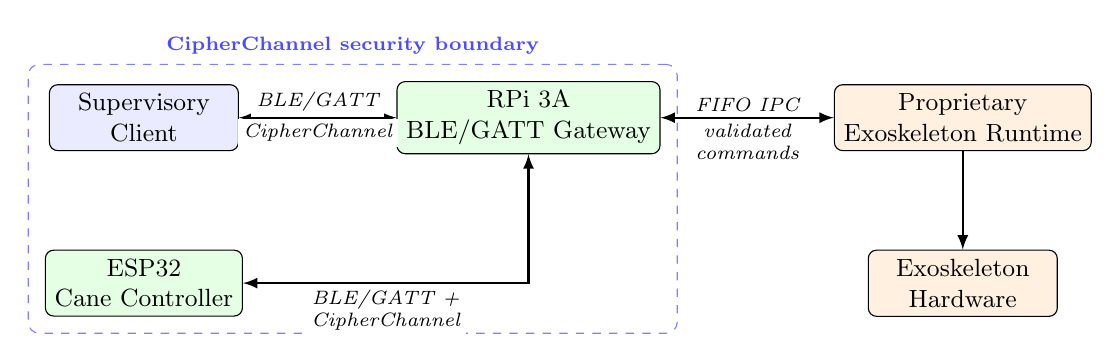
\begin{tikzpicture}[
  node distance = 0.5cm and 0.8cm,
  box/.style    = {draw, rounded corners=3pt, minimum width=2.4cm,
                   minimum height=0.75cm, font=\small, align=center,
                   fill=blue!8},
  cloud/.style  = {draw, rounded corners=3pt, minimum width=2.4cm,
                   minimum height=0.75cm, font=\small, align=center,
                   fill=orange!12},
  hw/.style     = {draw, rounded corners=3pt, minimum width=2.4cm,
                   minimum height=0.75cm, font=\small, align=center,
                   fill=green!10},
  arr/.style    = {-latex, thick},
  darr/.style   = {latex-latex, thick},
  elabel/.style = {font=\scriptsize\itshape, midway, fill=white,
                   inner sep=2pt, align=center}
]

\node[box] (client) {Supervisory\\Client};
\node[hw, right=2.0cm of client] (rpi) {RPi~3A\\BLE/GATT Gateway};
\node[cloud, right=2.2cm of rpi] (runtime) {Proprietary\\Exoskeleton Runtime};
\node[hw, below=1.25cm of client] (cane) {ESP32\\Cane Controller};
\node[cloud, below=1.25cm of runtime] (exo) {Exoskeleton\\Hardware};

\draw[darr] (client.east) -- node[elabel, above]{BLE/GATT}
                             node[elabel, below]{CipherChannel} (rpi.west);
\draw[darr] (cane.east) -| node[elabel, below, pos=0.25]{BLE/GATT +\\CipherChannel}
                           (rpi.south);
\draw[darr] (rpi.east) -- node[elabel, above]{FIFO IPC}
                           node[elabel, below]{validated\\commands} (runtime.west);
\draw[arr]  (runtime.south) -- (exo.north);

\begin{pgfonlayer}{background}
  \node[draw=blue!50, dashed, rounded corners=4pt, inner sep=6pt,
        fit=(client)(cane)(rpi),
        label={[font=\scriptsize\bfseries, text=blue!70]above:%
               CipherChannel security boundary}] {};
\end{pgfonlayer}

\end{tikzpicture}%
}
\caption{Gateway mediated command boundary. CipherChannel protects BLE/GATT traffic between the supervisory client or cane and the gateway. The proprietary exoskeleton runtime receives only commands that have passed application layer authentication, replay validation, direction validation, and persistent counter-state update.}
\label{fig:architecture}
\end{figure}

\subsection{Evaluated Exoskeleton Integration}

The supervisory client represents the operator-facing control endpoint. In a deployment, this may be a mobile application used by a clinician or authorised user to initiate high-level operational commands such as \texttt{STAND\_UP}, \texttt{START\_WALKING}, \texttt{TAKE\_STEP}, \texttt{STOP\_ACTION}. In the experiments, the mobile application was replaced by a laptop running a Python/Bleak client to provide repeatable timing instrumentation and structured logs. This substitution changes only the BLE client implementation; the GATT writes, CipherChannel packet format, gateway validation path, and runtime forwarding logic remain the same.

The Raspberry~Pi~3A gateway terminates BLE/GATT communication and enforces the CipherChannel admission rule. It runs Raspbian OS, Python~3, BlueZ, and the \texttt{bless} GATT server library. The gateway exposes command, notification, and security-provisioning characteristics for the supervisory client and cane paths.

The ESP32 auxiliary cane controller represents a second authorised endpoint. It scans for the gateway service UUID, connects as a BLE central, and writes encrypted cane-trigger events to the gateway. The cane implementation uses Arduino~C++ with mbedTLS and persists its CipherChannel state in ESP32 Non-Volatile Storage. A hardware button clears the stored key and triggers re-provisioning.

The proprietary exoskeleton runtime is treated as an external command consumer. It does not parse CipherChannel packets, maintain cryptographic state, or participate in BLE security. It receives only raw validated action strings from the gateway over named FIFO pipes.

\subsection{Command Flow and Runtime Isolation}

A command follows a five stage path. First, the supervisory client or cane serialises a high-level action into a compact UTF-8 payload. During experiments, the payload also includes an optional trial identifier used only for measurement:

\begin{verbatim}
{"trial_id":"t0001", "action":"STAND_UP"}
\end{verbatim}

Second, the endpoint encrypts the payload using CipherChannel and writes the resulting \texttt{nonce || ciphertext || tag} packet to the appropriate GATT characteristic. Freshness is not encoded in the JSON payload; it is encoded in the persistent counter nonce carried in the CipherChannel packet header.

Third, the gateway receives the complete encrypted byte buffer from the BLE host stack and applies CipherChannel validation. The gateway verifies the AES-GCM tag, checks that the counter is strictly greater than the last accepted counter for that logical endpoint, checks the expected direction parity, and persists
the new receive counter before exposing the plaintext command to the rest of the gateway logic.

Fourth, only after successful validation does the gateway enqueue the raw action string for the runtime-facing thread. Invalid packets are rejected before FIFO forwarding and do not produce runtime-visible commands.

Fifth, the gateway writes the validated action to the outgoing FIFO connected to the proprietary runtime. Runtime responses are read from the return FIFO and published to the appropriate BLE notification path. This preserves a narrow runtime interface: the runtime receives the same type of high-level action string it would receive without CipherChannel, while the security-sensitive packet parsing and replay state remain isolated inside the gateway.


\subsection{Endpoint Roles and State Separation}

The gateway maintains separate CipherChannel contexts for the supervisory client path and the cane path. Each context has its own send counter, receive counter, direction parity, and replay state. This prevents a valid packet from one logical endpoint path from being accepted as fresh traffic on another path. The separation is particularly important because the supervisory client and the cane can both communicate with the same gateway during the same operational window.

Operationally, the supervisory client initiates high-level mode changes, while the cane may later continue or interrupt execution through user triggered events. Both paths are subject to the same command admission rule: a command is forwarded to the runtime only after CipherChannel authentication, freshness validation, direction validation, and replay state persistence.

% \subsection{Implementation Notes}

% The gateway uses three main execution paths. A BLE/GATT thread drives the
% \texttt{bless} server event loop. A gateway to runtime thread dequeues validated
% commands and writes them to the outgoing FIFO. A runtime to gateway thread reads
% responses from the return FIFO and routes them to BLE notifications. These
% threads communicate through bounded queues, so the cryptographic validation path
% does not share mutable command buffers directly with the runtime forwarding
% path.

% Before writing a command to the outgoing FIFO, the gateway checks whether the
% runtime process is active. Commands received while the runtime process is absent
% are discarded with a logged warning rather than queued for later execution. This
% choice avoids releasing stale commands after a runtime restart and keeps replay
% control inside CipherChannel rather than in runtime-side buffering.

% The architecture deliberately keeps implementation-specific details below the
% protocol abstraction. The Raspberry~Pi, BlueZ, \texttt{bless}, FIFO, and ESP32
% details are used to make the evaluation reproducible, but the research
% contribution is the gateway mediated command authentication boundary and the
% CipherChannel protocol enforced at that boundary.

% BEGIN COMMENTED OUT: Operational control-flow figure removed to save space
% \begin{figure}[!t]
% \centering
% \resizebox{\columnwidth}{!}{%
% \begin{tikzpicture}[
%   x=1cm,y=1cm,
%   participant/.style={draw, rounded corners=2pt, fill=gray!10, minimum width=2.4cm, minimum height=0.55cm, font=\scriptsize, align=center},
%   lifeline/.style={gray!70, dashed},
%   msg/.style={-Latex, thick},
%   note/.style={draw, rounded corners=2pt, fill=yellow!12, font=\scriptsize, align=left, inner sep=3pt}
% ]
% \node[participant] (p) at (0,0) {Phone app};
% \node[participant] (c) at (3.4,0) {Cane};
% \node[participant] (r) at (6.8,0) {RPi middleware};
% \node[participant] (a) at (10.2,0) {Exoskeleton runtime};
% \draw[lifeline] (0,-0.35) -- (0,-6.2);
% \draw[lifeline] (3.4,-0.35) -- (3.4,-6.2);
% \draw[lifeline] (6.8,-0.35) -- (6.8,-6.2);
% \draw[lifeline] (10.2,-0.35) -- (10.2,-6.2);
% \draw[msg] (0,-1.0) -- (6.8,-1.0) node[midway, above, font=\scriptsize]{select mode + GO};
% \draw[msg] (6.8,-1.7) -- (10.2,-1.7) node[midway, above, font=\scriptsize]{forward mode command via FIFO};
% \draw[msg] (10.2,-2.4) -- (6.8,-2.4) node[midway, above, font=\scriptsize]{ready / state update};
% \draw[msg] (6.8,-3.1) -- (0,-3.1) node[midway, above, font=\scriptsize]{status notify};
% \node[note] at (1.7,-4.0) {Execution may\\transfer to cane};
% \draw[msg] (3.4,-4.7) -- (6.8,-4.7) node[midway, above, font=\scriptsize]{trigger / hold / release};
% \draw[msg] (6.8,-5.4) -- (10.2,-5.4) node[midway, above, font=\scriptsize]{forward cane action or interruption};
% \draw[msg] (10.2,-6.1) -- (6.8,-6.1) node[midway, below, font=\scriptsize]{ack / telemetry / error};
% \end{tikzpicture}%
% }
% \caption{Operational control flow. A supervisory client may initiate a mode,
% whereas execution can later be continued or interrupted through the auxiliary
% cane. The gateway mediates both flows and forwards only validated commands to
% the exoskeleton runtime.}
% \label{fig:opflow}
% \end{figure}
% END COMMENTED OUT: Operational control-flow figure removed to save space

% ---------------------------------------------------------------
\section{The CipherChannel Protocol}
\label{sec:protocol}
% ---------------------------------------------------------------

\subsection{Threat Model}
\label{sec:threatmodel}

We adopt the following adversarial model for the wireless command channel between the supervisory client / cane controller and the RPi gateway.

\paragraph{In-scope threats}
\begin{itemize}
  \item \textbf{Passive eavesdropping}: An adversary captures BLE radio frames.
  \item \textbf{Replay attack}: A captured valid ciphertext is retransmitted to trigger an unintended exoskeleton movement.
  \item \textbf{Message modification}: An intercepted ciphertext is altered before delivery, attempting to corrupt or substitute a command.
  \item \textbf{Session hijacking / MITM}: An adversary attempts to inject frames into an established BLE session (cf.\ InjectaBLE).
  \item \textbf{Key disclosure}: Long-term transport key material stored on a compromised device is used to impersonate a legitimate client.
  \item \textbf{Stale-session attack}: A client that has lost synchronisation with the gateway attempts to re-use an expired cipher context.
\end{itemize}

\paragraph{Out-of-scope threats}
Physical compromise of the gateway hardware, side channel attacks on the cryptographic implementation, and denial-of-service attacks against the BLE radio are considered out of scope. Compromise of an authorised endpoint before command generation (e.g., capturing valid encrypted packets from a compromised client for later replay) is also out of scope; CipherChannel assumes the endpoint is trusted at the time of command creation. Authentication of the user or clinician operating the endpoint is handled by higher-level policies and is not part of the protocol.

\subsection{Cryptographic Primitives}

CipherChannel is built on AES-256-GCM, a nonce-based authenticated encryption with associated data (AEAD) scheme specified by NIST SP~800-38D~\cite{nist_sp800_38d}. AEAD is required for the command channel considered here because confidentiality alone is insufficient: the receiver must also authenticate the origin and integrity of each command before releasing it to the exoskeleton runtime. The 128-bit GCM authentication tag provides integrity protection for the short command payloads used by the gateway.

AES-GCM was selected because it is standardised, widely implemented in embedded and server-side cryptographic libraries, and provides confidentiality, integrity, and authenticity in a single primitive. Prior embedded-security studies have also shown that AES-family primitives remain practical on low-end IoT hardware and Raspberry~Pi-class platforms, although performance depends strongly on hardware acceleration, implementation language, and cryptographic-library support~\cite{kietzmann2021hw,riddle2023aespie}. This choice is not intended to imply that AES-GCM is always the fastest AEAD scheme on every embedded platform. On software-only embedded targets without hardware AES acceleration, ChaCha20-Poly1305 has been reported to outperform AES-GCM substantially; for example, De Santis and Sigl report a 12.9$\times$ cycle-count advantage over AES-GCM on an ARM Cortex-M4 platform~\cite{desantis2017chacha20}. This comparison is relevant for microcontrollers without AES acceleration, but it does not directly determine the bottleneck in the evaluated CipherChannel path.

In CipherChannel, command payloads are short, typically consisting of compact JSON action objects. Under the tested conditions, AES-256-GCM authentication and decryption were not the dominant source of command latency; BLE transport scheduling and durable receive-counter persistence contributed more to the measured command path, as shown in Section~\ref{sec:eval}. Therefore, while ChaCha20-Poly1305 remains a reasonable alternative for platforms without AES acceleration, AES-256-GCM is suitable for the evaluated Raspberry~Pi gateway path and for embedded targets that provide efficient AES support.

For CipherChannel, the primary cryptographic requirement is nonce uniqueness under a fixed operational key. The persistent 96-bit counter-nonce construction in Section~\ref{sec:counternonce} is designed to satisfy this requirement across disconnections and process restarts. The AEAD primitive may be revisited for future ports whose hardware accelerators, cryptographic libraries, or certification requirements differ from the evaluated implementation.

\subsection{Packet Format}
\label{sec:packetformat}

Each CipherChannel packet transmitted over a BLE GATT write or notification has
three fields:

\[
\underbrace{\text{CtrNonce}}_{12\,\text{B}} \parallel
\underbrace{\text{Ciphertext}}_{n\,\text{B}} \parallel
\underbrace{\text{Tag}}_{16\,\text{B}}
\]

\noindent where \emph{CtrNonce} is a 96-bit little-endian counter value used as the AES-GCM nonce, \emph{Ciphertext} is the encrypted application payload, and \emph{Tag} is the 128-bit GCM authentication tag. Freshness is encoded directly in the counter nonce rather than in plaintext sequence or timestamp fields. The nonce is public, unique, monotonically increasing per direction, and authenticated by AES-GCM as part of tag verification. The protocol uses the conventional 96-bit AES-GCM IV size recommended for the efficient GCM construction~\cite{nist_sp800_38d}. After even/odd direction coding, each direction still has a usable nonce space of $2^{95}$ packets per operational key, which is far beyond the lifetime command volume of the target exoskeleton deployment.

The plaintext protected by AES-GCM is a UTF-8 encoded application payload. In the evaluated implementation, this payload is a compact JSON command object containing the requested action and, during experiments, an optional trial identifier used only for measurement. A representative payload is \texttt{{"trial\_id":"t0001", "action":"STAND\_UP"}}. The protocol does not rely on JSON-specific semantics: CipherChannel treats the encoded payload as an opaque byte string and provides confidentiality, integrity, and replay protection for the complete byte sequence.

AES-GCM supports arbitrary-length plaintexts and therefore does not require block padding. Consequently, the CipherChannel packet contains only the 96-bit counter nonce, the ciphertext corresponding to the encoded payload, and the 128-bit authentication tag. Freshness is not stored inside the JSON object; it is provided by the persistent counter nonce carried in the packet header.


\subsection{Handling BLE MTU Constraints}
\label{sec:mtu}

A CipherChannel packet has 28~bytes of fixed cryptographic overhead: 12~bytes for the counter nonce and 16~bytes for the AES-GCM authentication tag. Freshness is encoded in the persistent 96-bit counter nonce, so the packet does not carry separate plaintext sequence-number or timestamp fields. With the default BLE ATT MTU of 23~bytes, approximately 20~bytes are available for the attribute value after ATT headers. Therefore, even short encrypted commands may exceed the payload size of a single default-MTU GATT write.

The evaluated implementation passes the complete CipherChannel frame to the BLE host stack and relies on the behaviour provided by the client library, BlueZ, and the GATT implementation, including long-write handling or stack-level segmentation where available. This design choice does not affect the cryptographic validation rule. The gateway applies CipherChannel processing only after receiving a complete encrypted byte buffer. The buffer is then parsed as \texttt{CtrNonce || Ciphertext || Tag}; AES-GCM authentication is verified; counter monotonicity and direction parity are checked; the accepted receive counter is persisted; and only then is the plaintext command forwarded to the runtime interface.

For BLE stacks that do not transparently carry frames larger than the effective ATT payload, CipherChannel can use a simple application level fragmentation profile above GATT. In this profile, the sender first constructs the complete CipherChannel frame and then splits it into fragments. Each fragment carries a small plaintext reassembly header, for example \texttt{frame\_id}, \texttt{frag\_index}, \texttt{frag\_count}, and \texttt{total\_len}, followed by a fragment of the opaque CipherChannel frame. The receiver buffers fragments with the same \texttt{frame\_id}, rejects duplicate or out-of-range fragment indexes, enforces the configured maximum frame size, and discards incomplete reassembly state after a timeout. No fragment is decrypted or released to the application independently; AES-GCM verification, replay validation, direction validation, and receive-counter persistence are performed only after the full CipherChannel frame has been reassembled.

To characterise the evaluated BLE path, we performed an MTU/long-write confirmation experiment from the laptop/Bleak client to the Raspberry~Pi/BlueZ gateway. The backend exposed a negotiated ATT MTU of 23~bytes, but the evaluated BlueZ/Bleak path still accepted complete CipherChannel frames larger than the default 20-byte ATT value. Encrypted frames succeeded up to a 400-byte plaintext command, corresponding to a 428-byte CipherChannel frame, while a 512-byte plaintext command, corresponding to a 540-byte encrypted frame, failed.

This result confirms that the evaluated stack can carry the command sized encrypted frames used in our experiments. It should not be interpreted as a portable guarantee across BLE stacks. The fragmentation profile above provides a compatibility path for heterogeneous mobile operating systems, microcontroller BLE stacks, or larger payloads, but it was not exercised in the reported evaluation.


\subsection{Persistent Counter Nonces and Replay Protection}
\label{sec:counternonce}

CipherChannel uses the AES-GCM nonce as the only freshness and replay control metadata. Each endpoint maintains two persistent 96-bit counters: one for messages it sends and one recording the highest valid counter it has received from its peer. The state file contains the operational key and both counters and is updated atomically using a temporary file followed by \texttt{os.replace()}, so a crash cannot leave a partially written state file.

The two traffic directions are separated by counter parity. During channel creation, exactly one endpoint is marked as the initiator. The initiator sends only even counter values, while the non-initiator sends only odd counter values:

\begin{equation}
\mathit{ctr}_{send} \leftarrow \mathit{ctr}_{send} + 2,
\qquad
\mathit{nonce} = \mathit{ctr}_{send}.
\label{eq:sendcounter}
\end{equation}

\noindent The send counter is persisted before the encrypted packet is returned to the caller. This ordering prevents nonce reuse after a crash between packet construction and physical transmission. Reusing a GCM nonce under the same key would violate AES-GCM security, so this write-before-send rule is a security-critical implementation requirement.

If authentication succeeds, it interprets the nonce as a little-endian integer $c$ and accepts the message only if the counter is fresh and belongs to the expected receive-direction parity class:

\begin{equation}
c > \mathit{ctr}_{recv}
\quad\land\quad
(c \bmod 2) = \mathit{parity}_{recv}.
\label{eq:counteraccept}
\end{equation}

\noindent The receiver then persists $c$ as the new highest received counter \emph{before} returning the plaintext command to the gateway logic. This ordering prevents replay after a crash occurring between successful decryption and command execution. A replayed packet has $c \leq \mathit{ctr}_{recv}$ and is therefore rejected. A packet reflected back to its sender has the wrong parity and is also rejected. A packet modified in transit fails GCM tag verification before any counter update is attempted.

The counter-nonce construction does not require wall clock stamps, timing windows, sliding replay windows, or an unauthenticated reset transition. Missed packets do not cause permanent desynchronisation because the receiver accepts any higher same-parity counter. The protocol does not, however, acknowledge delivery: an attacker can still suppress BLE packets or cause denial of service. Delivery confirmation and retry policy therefore remain application layer responsibilities.

Counter state must never be reset under the same operational key. Reinitialising counters to zero is safe only when a fresh operational key is generated during a new provisioning event. If the same operational key is reused, the endpoint must load the existing persistent state rather than recreate the channel.

Replay resistant authentication and lightweight rekeying have also been studied for healthcare BLE and IoT-edge settings, further supporting the need for freshness and key lifecycle mechanisms above the wireless link layer ~\cite{rakshit2025dsekp}.

\begin{algorithm}[!t]
\caption{Counter-Nonce CipherChannel Send and Receive}
\label{alg:counternonce}
\footnotesize
\begin{algorithmic}[1]
\Require Operational key $K_S$; persistent state $(ctr_s, ctr_r, parity_s, parity_r)$
\Ensure Valid packets are decrypted once; invalid or replayed packets return $\bot$
\Function{Send}{$m$}
  \State $ctr_s \leftarrow ctr_s + 2$
  \If{$ctr_s \geq 2^{96}$} \State \Return provisioning required \EndIf
  \State Persist $ctr_s$ for the current key version and channel
  \State $N \leftarrow \textsc{LE}_{96}(ctr_s)$
  \State $(C,T) \leftarrow \textsc{AESGCM.Enc}_{K_S}(N,m)$
  \State \Return $N \| C \| T$
\EndFunction
\Statex
\Function{Receive}{$N \| C \| T$}
  \State $c \leftarrow \textsc{LE}^{-1}_{96}(N)$
  \If{$c \leq ctr_r$ or $(c \bmod 2) \neq parity_r$} \State \Return $\bot$ \EndIf
  \State $m \leftarrow \textsc{AESGCM.Dec}_{K_S}(N,C,T)$
  \If{$m = \bot$} \State \Return $\bot$ \EndIf
  \State Persist $ctr_r \leftarrow c$ for the current key version and channel
  \State \Return $m$
\EndFunction
\end{algorithmic}
\end{algorithm}

\subsection{Security Invariant}
\label{sec:securityinvariants}

For a fixed operational key and logical channel, CipherChannel ensures nonce uniqueness, replay rejection, reflection rejection, and modification/injection resistance, assuming correct persistent-state handling and standard AES-GCM security. Nonce uniqueness follows because the send counter is increased by two and persisted before packet transmission, while the two traffic directions use disjoint parity classes. Replay resistance follows because a receiver accepts only counters that are strictly greater than the last persisted receive counter and stores the new counter before exposing the plaintext command to the gateway. Reflection attacks are rejected because packets generated in one direction have the wrong parity when injected into the opposite receive path. Finally, packet modification or injection succeeds only if the adversary can forge a valid AES-GCM tag under the operational key. Thus, an attacker who observes, replays, reorders, reflects, or modifies BLE frames cannot cause the gateway to accept an unauthorised command except with negligible AES-GCM forgery probability.

\subsection{Dual-Key Architecture}
\label{sec:dualkey}

CipherChannel separates bootstrap authorization from operational command
protection. The protocol uses two classes of key material:

\begin{itemize}
  \item \textbf{Transport Key} ($K_T$): a static 256-bit pre-shared bootstrap key installed at provisioning time on the gateway and on authorised controller endpoints. $K_T$ is used only to protect the operational key during the provisioning exchange in Section~\ref{sec:keyexchange}; it is not used for normal exoskeleton commands.
  \item \textbf{Operational Keys} ($K_{S,phone}$ and $K_{S,cane}$): endpoint-specific 256-bit keys used for authenticated encryption of operational command traffic. Each authorised endpoint obtains its own operational key during a physically gated exchange. The gateway maintains separate cipher contexts for the supervisory client path and the cane-controller path; each context has its own operational key, send counter, receive counter, parity role, and replay state.
\end{itemize}

This separation ensures that BLE pairing success is not sufficient for command authorisation. An accepted command must be protected under the endpoint-specific operational key for its logical channel and must satisfy AEAD verification, counter-monotonicity validation, and direction-parity checks. The packet format is unchanged by endpoint-specific keying because key selection is determined by the GATT characteristic and logical endpoint context rather than by an additional packet field.

\subsection{Physical-Presence-Gated Key Exchange}
\label{sec:keyexchange}

Key exchange is the process by which a client acquires its endpoint-specific operational key $K_{S,e}$ from the gateway over BLE. The protocol is described in
Algorithm~\ref{alg:keyex}.

\begin{algorithm}[!t]
\caption{CipherChannel Key Exchange Protocol}
\label{alg:keyex}
\footnotesize
\begin{algorithmic}[1]
\Require Client and gateway share $K_T$; gateway holds endpoint-specific $K_{S,e}$ for endpoint $e$
\Ensure  Client acquires $K_{S,e}$ encrypted under $K_T$
\State \textbf{Gateway:} Operator physically presses button on gateway hardware
\State \textbf{Gateway:} $\mathit{button\_pressed} \leftarrow \text{True}$;
       start provisioning timer $\tau$ (configured to 60\,s)

\State \textbf{Client:} Write \texttt{REQUEST\_KEY} to Security characteristic

\If{$\mathit{button\_pressed}$ and $\tau$ not expired}
  \State \textbf{Gateway:} $c_{K_S} \leftarrow
         \text{CipherChannel}_{K_T}.\text{encrypt}(K_S)$
  \State \textbf{Gateway:} Write $c_{K_S}$ to Security characteristic
  \State \textbf{Client:} $K_S \leftarrow
         \text{CipherChannel}_{K_T}.\text{decrypt}(c_{K_S})$
  \State \textbf{Client:} Store $K_S$ and initialise persistent counter state
  \State \textbf{Client:} Write \texttt{STOP\_SHARING} to Security characteristic
  \State \textbf{Gateway:} Overwrite Security characteristic with
         $\text{CipherChannel}_{K_T}.\text{encrypt}(\texttt{WAITING})$
  \State \textbf{Gateway:} $\mathit{button\_pressed} \leftarrow \text{False}$
\Else
  \State \textbf{Gateway:} No response; key not transmitted
\EndIf
\end{algorithmic}
\end{algorithm}

% \begin{figure}[!t]
% \centering
% \resizebox{\columnwidth}{!}{%
% \begin{tikzpicture}[
%   x=1cm,y=1cm,
%   participant/.style={draw, rounded corners=2pt, fill=gray!10, minimum width=2.9cm, minimum height=0.55cm, font=\scriptsize, align=center},
%   lifeline/.style={gray!70, dashed},
%   msg/.style={-Latex, thick},
%   reply/.style={-Latex, thick, dashed}, % Added for dashed return lines
%   note/.style={draw, rounded corners=2pt, fill=yellow!12, font=\scriptsize, align=left, inner sep=3pt}
% ]

% % Participants
% \node[participant] (c) at (0,0) {Phone or Cane};
% \node[participant] (r) at (4.6,0) {RPi middleware};
% \node[participant] (a) at (9.2,0) {CT-AWAKE};

% % Lifelines (extended to -11.5)
% \draw[lifeline] (0,-0.35) -- (0,-11.5);
% \draw[lifeline] (4.6,-0.35) -- (4.6,-11.5);
% \draw[lifeline] (9.2,-0.35) -- (9.2,-11.5);

% % Messages
% \draw[msg] (0,-1.0) -- (4.6,-1.0) node[midway, above, font=\scriptsize]{BLE connect};
% \node[note, anchor=west] at (0.25,-1.8) {Secure exchange allowed only in\\safe-environment window};
% \draw[msg] (0,-2.7) -- (4.6,-2.7) node[midway, above, font=\scriptsize]{\texttt{REQUEST\_KEY} on security characteristic};
% \draw[reply] (4.6,-3.6) -- (0,-3.6) node[midway, above, font=\scriptsize, align=center]{deployment-specific operational key\\over bootstrap channel};
% \draw[msg] (0,-4.5) -- (4.6,-4.5) node[midway, above, font=\scriptsize]{\texttt{STOP\_SHARING}};
% \draw[reply] (4.6,-5.4) -- (0,-5.4) node[midway, above, font=\scriptsize, align=center]{security characteristic cleared\\/ sharing window closed};
% \draw[reply] (4.6,-6.3) -- (0,-6.3) node[midway, above, font=\scriptsize, align=center]{persistent counters initialised\\or loaded};
% \draw[reply] (4.6,-7.2) -- (0,-7.2) node[midway, above, font=\scriptsize]{operational secure channel ready};
% \draw[msg] (0,-8.1) -- (4.6,-8.1) node[midway, above, font=\scriptsize]{encrypted action command};
% \draw[msg] (4.6,-9.0) -- (9.2,-9.0) node[midway, above, font=\scriptsize]{FIFO write};
% \draw[reply] (9.2,-9.9) -- (4.6,-9.9) node[midway, above, font=\scriptsize]{ack / state / telemetry};
% \draw[reply] (4.6,-10.8) -- (0,-10.8) node[midway, above, font=\scriptsize]{encrypted notify / update};
% \end{tikzpicture}%
% }
% \caption{Provisioning and secure-channel establishment sequence. The gateway
% releases the deployment-specific operational key only during a physically enabled,
% safe-environment window, after which normal encrypted control traffic can
% proceed.}
% \label{fig:keyex}
% \end{figure}


The exchange keeps $K_S$ confidential by wrapping it under AES-256-GCM with $K_T$, releases it only during a physically enabled provisioning window, and clears the security characteristic after \texttt{STOP\_SHARING}. Timeout handling closes incomplete exchanges, and fresh counter state is initialised only with a fresh operational key; otherwise, stored counters must be reloaded to avoid AES-GCM nonce reuse.

The confidentiality of $K_S$ follows from the IND-CCA security of AES-GCM under the temporary provisioning key $K_T$.
An adversary that does not know $K_T$ can observe the encrypted provisioning response, but cannot recover $K_S$ or modify the ciphertext into another valid response without causing authentication failure.
The provisioning window is also explicitly bounded: it expires after 60~s, accepts only a single response, and is cleared after \texttt{STOP\_SHARING}.
Consequently, a captured provisioning ciphertext is not accepted as a fresh provisioning response when the provisioning channel preserves its CipherChannel counter state under $K_T$: replayed provisioning packets fail the same monotonic counter and direction-parity checks as operational packets. The one-shot provisioning window and \texttt{STOP\_SHARING} clearing reduce exposure of the key transfer characteristic, but replay resistance relies on authenticated encryption together with persistent provisioning-channel counters.

% BEGIN COMMENTED OUT: Expanded key exchange property list compressed to save space
% \noindent\textbf{Security properties of the exchange.}
% The key exchange protocol provides the following guarantees:
%
% \begin{enumerate}
%   \item \textbf{Confidentiality of $K_S$}: $K_S$ is never transmitted in
%     plaintext; it is wrapped under AES-256-GCM with $K_T$.
%   \item \textbf{Physical presence requirement}: The provisioning timer is only
%     started by a physical button press at the gateway. An adversary who has
%     compromised $K_T$ remotely cannot extract $K_S$ without physical access
%     to the gateway.
%   \item \textbf{Single-use transmission}: After the client sends
%     \texttt{STOP\_SHARING}, the gateway overwrites the characteristic with
%     an encryption of the sentinel string \texttt{WAITING}, destroying the
%     ciphertext of $K_S$ from the BLE attribute cache.
%   \item \textbf{Timeout}: If the exchange is not completed before the provisioning timer expires, the gateway resets the button-pressed flag
%     and will not respond to any subsequent \texttt{REQUEST\_KEY} until a
%     new button press occurs.
%   \item \textbf{Counter-state initialisation}: A newly provisioned operational
%     key is associated with fresh persistent send/receive counters. Counter
%     reinitialisation is permitted only together with a fresh operational key;
%     otherwise stored counter state must be loaded to avoid AES-GCM nonce reuse.
% \end{enumerate}
% END COMMENTED OUT: Expanded key exchange property list compressed to save space



\subsection{Eliminating Explicit Reset Semantics}
\label{sec:reset}
The counter-nonce design removes the need for an explicit reset characteristic. The receiver accepts any strictly greater counter of the correct direction parity, so ordinary packet loss, disconnection, and reconnection do not by themselves require a state reset.

This simplifies both the protocol and the security argument. A BLE reconnection does not create a new CipherChannel session; both endpoints reload their persistent counter state and continue from the last stored values. A replayed pre-disconnection packet is rejected because its counter is not greater than the stored receive counter. A reflected packet is rejected because it has the wrong direction parity. A forged reset request is not an attack vector because the protocol contains no unauthenticated reset transition.

If an endpoint loses or corrupts its persistent state, the secure recovery path is to perform a new physically gated provisioning event that installs a fresh operational key and fresh counters. Recreating counters under the same key is forbidden, because it could repeat an AES-GCM nonce.

% ---------------------------------------------------------------
\section{Reference Implementation}
\label{sec:impl}

The reference implementation includes a Python/PyCryptodome gateway implementation and an ESP32/mbedTLS cane-endpoint implementation. The packet format is library-independent and is defined by the \texttt{nonce || ciphertext || tag} layout, the 96-bit counter nonce, and the receive-side monotonicity and direction-parity checks. The reference implementation and experiment artefacts are publicly available under the Apache-2.0 license at \url{https://github.com/thodpap/CipherChannel}.

\subsection{Implementation Robustness}
\label{sec:impl-robustness}

The implementation treats CipherChannel state as security-critical shared state rather than as ordinary application metadata. On the Raspberry~Pi gateway, cryptographic contexts, send counters, receive counters, and endpoint-specific key material are protected by Python locks so that BLE callbacks, runtime forwarding threads, and notification paths cannot concurrently mutate replay state. On the ESP32 cane endpoint, the corresponding state transitions are guarded by FreeRTOS synchronization primitives. This prevents concurrent command handling from producing duplicate send counters, stale receive-counter updates, or inconsistent endpoint state.

Crash safe persistence is enforced through ordered state updates. Send counters are made durable before encrypted packets are returned for transmission, preventing AES-GCM nonce reuse after a crash between packet construction and physical delivery. Receive counters are made durable before plaintext commands are released to the gateway logic, preventing a post-crash replay of an already accepted packet. On the Python gateway, state updates are written to a temporary file, flushed with \texttt{fsync}, and committed with atomic rename via \texttt{os.replace()}. This ordering is deliberately conservative: it adds measurable latency, but preserves the replay-safety invariant across process restarts.

The implementation also isolates keys and replay state per logical endpoint. The supervisory client path and the cane controller path use separate operational keys, counters, direction parity roles, and receive state records. As a result, a valid packet from one endpoint context is not accepted as fresh traffic in another endpoint context, even when both communicate with the same gateway during the same operational window.

The cross-platform implementation was designed to keep the protocol independent of a single language or cryptographic library. The gateway path uses Python and PyCryptodome on Raspberry~Pi/BlueZ, while the cane endpoint uses Arduino C++ and mbedTLS on ESP32 with non-volatile storage for persistent state. The evaluation in this paper focuses on the Python/Bleak client and Python/Raspberry~Pi gateway path for BLE latency and adversarial-rejection measurements. The ESP32 implementation is reported for firmware resource footprint in Section~\ref{sec:esp32-footprint}.


% ---------------------------------------------------------------
\section{Experimental Evaluation}
\label{sec:eval}
% ---------------------------------------------------------------

The evaluation is organised around four research questions.

\begin{itemize}
  \item \textbf{RQ1 -- Security rejection}: Does CipherChannel reject replay, ciphertext/tag tampering, stale counters, wrong keys, reflection, reordering, and cross endpoint injection before a command reaches the runtime?

  \item \textbf{RQ2 -- Persistence and provisioning}: Does the protocol preserve replay state through simulated restart and enforce the physical-presence-gated provisioning state machine?

  \item \textbf{RQ3 -- Measured command latency}: Under the tested BLE conditions, what latency is observed for steady-state command/ACK exchange, cold start operation, key exchange, and distance/obstruction scenarios?

  \item \textbf{RQ4 -- Local processing cost}: Is the command path dominated by BLE transport, cryptographic processing, or durable counter persistence?
\end{itemize}

The experiments deliberately separate protocol validation from BLE transport. Unit and adversarial tests exercise the CipherChannel state machine without relying on radio timing. BLE command path experiments measure the latency observed by a client communicating with the Raspberry~Pi gateway. Gateway internal measurements instrument the receive callback to separate packet parsing, freshness validation, AES-GCM authentication/decryption, persistent counter update, JSON parsing, and ACK publication.

\subsection{Experimental Setup}

The evaluation was conducted on a laptop client and a Raspberry~Pi BLE gateway. The client host used a 12th Gen Intel Core i7-12650H processor, Fedora Linux, Python~3.14.5, PyCryptodome~3.23.0, Bleak~3.0.2, BlueZ~5.86, and a USB BLE adapter. The gateway was implemented on a Raspberry~Pi BLE server using \texttt{bless}~0.3.0 and BlueZ~5.86. A Python/Bleak client was used instead of the mobile application in order to obtain repeatable timing measurements over a large number of trials, while preserving the same GATT write path, CipherChannel packet format, gateway validation logic, and command forwarding behaviour.

The maximum plaintext command size was 400B, producing a maximum CipherChannel packet size of 428B after adding the 12-byte counter nonce and 16-byte AES-GCM authentication tag. All reported latency values and percentiles were computed consistently across the recorded trials, and confidence intervals are reported where supported by the result artefacts.

The canonical BLE command path evaluation covers the Python/PyCryptodome implementation, the Raspberry~Pi BLE gateway path, the provisioning-gate state machine, and BLE client-to-gateway command exchange. It does not evaluate C/OpenSSL interoperability, ESP32/mbedTLS interoperability, physical Raspberry~Pi power-cycle recovery, long-duration soak behaviour, or clinical workflow execution. ESP32 firmware resource usage is reported separately in Section~\ref{sec:esp32-footprint} as a footprint measurement, not as an interoperability or latency validation.

\subsection{Security Analysis Against Known BLE Attacks}
\label{sec:attackcoverage}

The BLE attacks discussed in Section~\ref{sec:background} motivate the need for a command authentication boundary above the BLE link layer. CipherChannel does not attempt to repair the underlying BLE protocol or make the BLE stack immune to downgrade, impersonation, reconnection, injection, or implementation-level attacks. Instead, it reduces the security dependence placed on BLE by requiring every command to satisfy an independent application layer acceptance rule before it is forwarded to the exoskeleton runtime.

Attacks such as KNOB/TOPS~\cite{antonioli2020knob,zhang2020downgrade}, BIAS~\cite{antonioli2020bias}, BLESA~\cite{wu2020blesa}, SweynTooth~\cite{garbelini2020sweyntooth}, InjectaBLE~\cite{cayre2021injectable}, BLUFFS~\cite{antonioli2023bluffs}, and pairing downgrade or method-confusion attacks~\cite{tschirschnitz2021method} affect different parts of the Bluetooth security model, including key negotiation, peer authentication, reconnection, frame injection, session-key derivation, and BLE stack robustness. In the CipherChannel design, however, BLE connection state is not sufficient for command authorisation. A received packet is accepted only if it authenticates under the operational key, carries a strictly fresh counter nonce, satisfies the expected direction parity, and causes the persistent receive counter to be updated before plaintext command release.

This design means that a weakened or spoofed BLE connection may still deliver traffic to the gateway, but it cannot by itself produce a valid exoskeleton command. Tampered packets fail AES-GCM authentication, replayed packets fail the monotonic counter check, reflected packets fail the direction-parity rule, and packets generated without the operational key fail tag verification. The remaining residual risks are denial of service, BLE stack crashes, physical compromise, endpoint compromise before encryption, and platform-level implementation vulnerabilities. These risks are outside the cryptographic acceptance rule and require additional system hardening, monitoring, and deployment controls.



\subsection{Protocol Correctness and Provisioning Gate}

Table~\ref{tab:correctness} summarises the protocol correctness tests. The tested cases cover packet-length invariants, counter behaviour, malformed-input rejection, and a protocol test vector. All 52 tests passed. The results confirm that packet overhead is exactly 28\,B for plaintext sizes from 0 to 400\,B, ciphertext length equals plaintext length, the nonce is encoded as a 12-byte little-endian counter, direction parity is enforced, and the counter-exhaustion guard triggers before nonce reuse.

\begin{table}[!t]
\renewcommand{\arraystretch}{1.15}
\caption{Protocol Correctness Test Results}
\label{tab:correctness}
\centering
\scriptsize
\begin{tabular}{lccc}
\toprule
\textbf{Group} & \textbf{Purpose} & \textbf{Tests} & \textbf{Passed} \\
\midrule
A1 & Packet-length invariants & 15 & 15 \\
A2 & Counter behaviour & 21 & 21 \\
A3 & Malformed-input rejection & 13 & 13 \\
A4 & Protocol test vector & 3 & 3 \\
\midrule
\textbf{Total} & & \textbf{52} & \textbf{52} \\
\bottomrule
\end{tabular}
\end{table}

The provisioning-gate suite passed 28/28 tests. These tests cover closed-gate rejection, active-window acceptance for the intended endpoint, wrong-endpoint rejection during an active window, one-shot provisioning, timeout behaviour, gate closing after successful provisioning, re-opening after a completed exchange, independent phone/cane gates, and concurrent provisioning attempts. These are state-machine tests; physical button timing and GPIO behaviour were not measured in this run.

\subsection{Adversarial Rejection and Endpoint Isolation}

Table~\ref{tab:adversarial} summarises the adversarial-rejection suite. Across 534 replay, tampering, stale-counter, wrong-key, reflection, and reordering attempts, the system produced zero unexpected acceptances. In the reordering experiment, packets with counters 2, 6, and 8 were correctly accepted as fresh, while the later delivery of counter 4 after counter 6 was correctly rejected as stale. Thus, the test confirms that CipherChannel permits benign loss/reordering only when the received counter remains fresh, and rejects stale delivery once the receive counter has advanced.

Endpoint isolation was also validated by injecting packets generated for one logical endpoint into the other endpoint path. The gateway rejected these cross endpoint attempts before runtime forwarding because each endpoint context uses separate operational key material, replay state, and direction-parity expectations.

Together with the distance and obstruction experiments reported below, these results indicate that CipherChannel did not introduce additional command acceptance failure modes beyond those already caused by the underlying BLE connection. Encrypted packets were either accepted after successful authentication and freshness validation, or rejected deterministically for a protocol-level reason. Range related failures were observed as BLE connection, write, notification, or ACK-read failures rather than as ambiguous CipherChannel accept/reject behaviour.

\begin{table}[!t]
\renewcommand{\arraystretch}{1.15}
\setlength{\tabcolsep}{3pt} % Reduces white space between columns
\caption{Adversarial-Rejection Test Results}
\label{tab:adversarial}
\centering
\scriptsize
\begin{tabular}{>{\raggedright\arraybackslash}p{2.4cm} c c c c >{\raggedright\arraybackslash}p{2.6cm}}
\toprule
\textbf{Case} & \textbf{Att.} & \textbf{Acc.} & \textbf{Rej.} & \textbf{Unexp.} & \textbf{Interpretation} \\
\midrule
Exact replay, local & 100 & 0 & 100 & 0 & Previously accepted ciphertexts were rejected. \\
Exact replay, BLE end-to-end & 30 & 0 & 30 & 0 & Replay was rejected over the measured BLE path. \\
Replay after BLE reconnect & 30 & 0 & 30 & 0 & Reconnect did not reset receive-counter state. \\
Replay after simulated process restart & 30 & 0 & 30 & 0 & Reloaded state rejected post-restart replay. \\
Ciphertext/tag tampering & 120 & 0 & 120 & 0 & Modified packets failed authentication. \\
Wrong key / cross endpoint variants & 4 & 0 & 4 & 0 & Wrong-key traffic did not authenticate. \\
Direction reflection & 100 & 0 & 100 & 0 & Wrong parity rejected reflected packets. \\
Reordering 2$\rightarrow$6$\rightarrow$4$\rightarrow$8 & 120 & 90 & 30 & 0 & Fresh packets accepted; stale packet 4 rejected. \\
\midrule
\textbf{Total} & \textbf{534} & \textbf{90} & \textbf{444} & \textbf{0} & No unexpected command acceptance. \\
\bottomrule
\end{tabular}
\end{table}

A separate endpoint-isolation experiment tested whether packets from one logical endpoint path could be accepted by the other. The gateway performed cane and phone key exchange, provisioning distinct operational keys for the two logical endpoint paths. The test then injected 30 phone-encrypted packets into the cane channel and 30 cane-encrypted packets into the phone channel. All 60 cross endpoint injections were rejected, and one valid command per channel was accepted as a sanity check. In this canonical run, cross endpoint packets failed AES-GCM authentication because they were protected under the wrong endpoint-specific operational key. This result supports endpoint isolation for the tested gateway configuration.

\subsection{Steady-State and Cold Start Command Latency}

The latency experiments distinguish the normal steady-state case from cold start operation. In steady state, the BLE connection and CipherChannel state have already been established; the client repeatedly encrypts a \texttt{STAND\_UP} command, writes it over GATT, and waits for the ACK. In cold start operation, each trial repeats scanning, connection, key exchange, command encryption, BLE write, and ACK waiting.

Table~\ref{tab:steady_latency} reports the steady-state result. Across 1000 trials, all commands succeeded. The median client-observed command to-ACK latency was 169.6\,ms, with p95 of 170.7\,ms and p99 of 214.7\,ms. Client-side AES-GCM encryption had 0.215\,ms median latency and 0.408\,ms p99 latency, whereas BLE write and ACK waiting dominated the observed command path.

\begin{table}[!t]
\renewcommand{\arraystretch}{1.15}
\setlength{\tabcolsep}{4pt}
\caption{Steady-State Secure Command/ACK Latency for \texttt{STAND\_UP} (ms, $N=1000$)}
\label{tab:steady_latency}
\centering
\scriptsize
\begin{tabular}{@{} l ccccc @{}} 
\toprule
\textbf{Phase} & $\mu$ & \textbf{p50} & $\sigma$ & \textbf{p95} & \textbf{p99} \\
\midrule
Client encrypt & 0.232 & 0.215 & 0.058 & 0.354 & 0.408 \\
BLE write & 80.231 & 79.245 & 6.645 & 80.401 & 124.307 \\
ACK wait & 90.227 & 90.094 & 2.543 & 91.147 & 91.531 \\
Command$\rightarrow$ACK & 170.713 & 169.596 & 7.068 & 170.743 & 214.709 \\
\bottomrule
\end{tabular}
\end{table}

Table~\ref{tab:coldstart} reports the cold start result. Across 500 trials, all commands succeeded. The total cold start path had 4.62\,s median latency and 10.38\,s p99 latency. The command to-ACK part of the same cold start trials had 179.5\,ms median and 224.9\,ms p99 latency. The difference shows that scan, connection establishment, and key exchange dominate cold start operation, while the encrypted command/ACK exchange remains in the same order of magnitude as the steady-state case.

\begin{table}[!t]
\renewcommand{\arraystretch}{1.15}
\setlength{\tabcolsep}{3pt}
\caption{Cold Start Provisioning and First-Command Latency (ms, $N=500$)}
\label{tab:coldstart}
\centering
\scriptsize
\begin{tabular}{lccccc}
\toprule
\textbf{Phase} & $\mu$ & \textbf{p50} & $\sigma$ & \textbf{p95} & \textbf{p99} \\
\midrule
Scan & 1018.1 & 807.8 & 788.0 & 2656.9 & 4459.9 \\
Connect & 3412.9 & 2688.5 & 1218.2 & 5921.6 & 7947.6 \\
Key exchange & 437.7 & 399.6 & 83.9 & 578.0 & 846.6 \\
Command encrypt & 0.091 & 0.069 & 0.047 & 0.156 & 0.312 \\
BLE write & 90.3 & 89.0 & 7.5 & 90.8 & 134.5 \\
ACK wait & 90.9 & 90.1 & 6.3 & 91.2 & 135.1 \\
Command$\rightarrow$ACK & 181.3 & 179.5 & 9.7 & 181.3 & 224.9 \\
Total & 5050.1 & 4624.1 & 1502.0 & 7774.5 & 10384.6 \\
\bottomrule
\end{tabular}
\end{table}

\subsection{Gateway Internal Processing Cost}

Table~\ref{tab:server_processing} reports gateway internal processing for 1000 steady-state commands. The measured interval begins inside the GATT characteristic-write callback and ends when the ACK characteristic value has been set. AES-256-GCM authentication and decryption had 1.70\,ms median and 1.98\,ms p99 latency. Freshness and direction-parity validation were below 0.005\,ms at p99. However, the durable receive-counter write had 14.21\,ms median and 101.87\,ms p99 latency, making persistence the dominant local gateway cost.

\begin{table}[!t]
\renewcommand{\arraystretch}{1.12}
\caption{Gateway Side Receive-to-ACK Processing Breakdown (ms, $N=1000$)}
\label{tab:server_processing}
\centering
\resizebox{\columnwidth}{!}{%
\begin{tabular}{lccccc}
\toprule
\textbf{Phase} & $\mu$ & \textbf{p50} & $\sigma$ & \textbf{p95} & \textbf{p99} \\
\midrule
Packet parse & 0.0295 & 0.0289 & 0.0105 & 0.0314 & 0.0420 \\
Freshness + direction validation & 0.0032 & 0.0032 & 0.0031 & 0.0034 & 0.0045 \\
AES-256-GCM auth + decryption & 1.7082 & 1.6989 & 0.2089 & 1.8719 & 1.9765 \\
Receive-counter fsync & 20.0119 & 14.2125 & 16.5830 & 30.5376 & 101.8685 \\
JSON parse + action identification & 0.2955 & 0.2956 & 0.0248 & 0.3360 & 0.3474 \\
ACK characteristic update & 0.4918 & 0.4910 & 0.0489 & 0.5629 & 0.5907 \\
\midrule
\textbf{Gateway total} & \textbf{22.5402} & \textbf{16.8113} & \textbf{16.5719} & \textbf{33.2315} & \textbf{104.4857} \\
\bottomrule
\end{tabular}%
}
\end{table}

This result changes the interpretation of gateway side overhead. CipherChannel cryptographic processing is not the dominant cost, but crash safe  persistence is not negligible when implemented with synchronous state-file updates. The result supports the protocol's fail closed persistence rule, but it also shows that production deployments should engineer durable counter storage carefully.

\subsection{Key Exchange Latency}

Table~\ref{tab:key_exchange_latency} reports 500 key exchange trials. Each trial includes scan, connection, \texttt{REQUEST\_KEY} write, server processing, client decryption of the operational key, and client channel-state initialisation. All 500 trials succeeded. The key exchange portion from request write to decrypted key had 443.5\,ms median latency and 937.9\,ms p99 latency. Client-side decryption and state initialisation were sub-millisecond at p99; the measured key exchange latency is therefore dominated by BLE request/response timing and server-side publication of the encrypted key material. Physical button latency is excluded because the benchmark provisioning gate was used.

\begin{table}[!t]
\renewcommand{\arraystretch}{1.15}
\setlength{\tabcolsep}{3pt}
\caption{Key Exchange Latency (ms, $N=500$)}
\label{tab:key_exchange_latency}
\centering
\scriptsize
\begin{tabular}{lccccc}
\toprule
\textbf{Phase} & $\mu$ & \textbf{p50} & $\sigma$ & \textbf{p95} & \textbf{p99} \\
\midrule
Scan & 991.7 & 741.7 & 832.4 & 2581.5 & 3930.5 \\
Connect & 3674.0 & 3323.7 & 1414.3 & 6639.7 & 8033.0 \\
\texttt{REQUEST\_KEY} write & 363.3 & 352.6 & 92.6 & 488.3 & 847.4 \\
Server process & 92.2 & 90.9 & 8.7 & 92.4 & 136.3 \\
Client decrypt key & 0.303 & 0.238 & 0.639 & 0.336 & 0.513 \\
State initialisation & 0.028 & 0.019 & 0.021 & 0.047 & 0.129 \\
KEX total & 455.8 & 443.5 & 93.1 & 578.7 & 937.9 \\
\bottomrule
\end{tabular}
\end{table}

\subsection{Distance and Obstruction Sensitivity}

Two distance experiments were conducted. The first repeated full reconnect operation across five conditions: 0.5\,m line of sight, 1\,m line of sight, 2\,m line of sight, 4\,m line of sight, and 7\,m with a wall. Each condition used 200 trials, for 1000 total reconnect trials. All 1000 trials succeeded, with no failures at scan, connection, key exchange, write, or ACK stages.

\begin{table}[!t]
\renewcommand{\arraystretch}{1.12}
\caption{Distance Sensitivity with Full Reconnect per Trial (ms, $N=200$ per condition)}
\label{tab:distance_latency}
\centering
\resizebox{\columnwidth}{!}{%
\begin{tabular}{lccccccl}
\toprule
\textbf{Condition} & $\mu$ & \textbf{p50} & $\sigma$ & \textbf{p95} & \textbf{p99} & \textbf{Max} & \textbf{Successes} \\
\midrule
0.5\,m LOS & 4481.9 & 4303.7 & 1334.8 & 7051.8 & 8217.7 & 8444.4 & 200/200 \\
1\,m LOS & 4468.4 & 4258.3 & 1316.0 & 6823.8 & 7999.6 & 8804.1 & 200/200 \\
2\,m LOS & 4329.0 & 4124.2 & 1302.1 & 6646.8 & 8713.2 & 9164.2 & 200/200 \\
4\,m LOS & 5002.7 & 4731.5 & 1557.6 & 7560.2 & 9666.9 & 12988.4 & 200/200 \\
7\,m wall & 5561.2 & 4798.5 & 2359.1 & 10624.3 & 12686.4 & 16138.9 & 200/200 \\
\bottomrule
\end{tabular}%
}
\end{table}
The second distance experiment kept an established connection open and measured sustained write/ACK latency across 1\,m, 2\,m, 4\,m, and 7\,m-wall conditions, with 500 trials per condition. All 2000 trials succeeded. The median command to-ACK latency remained approximately 169.3--169.4\,ms across all conditions, while the 7\,m-wall condition increased the mean and tail latency, reaching 259.6\,ms p99 and 350.5\,ms maximum latency.

\begin{table}[!t]
\renewcommand{\arraystretch}{1.12}
% Reduce the space between columns globally for this table
\setlength{\tabcolsep}{3.5pt} 
\caption{Distance Sensitivity in Steady-State BLE Operation (ms, $N=500$ per condition)}
\label{tab:distance_steady}
\centering
\scriptsize
\begin{tabular}{lccccccl}
\toprule
\textbf{Condition} & $\mu$ & \textbf{p50} & $\sigma$ & \textbf{p95} & \textbf{p99} & \textbf{Max} & \textbf{Succ.} \\
\midrule
1\,m LOS & 170.8 & 169.3 & 8.4 & 170.2 & 214.2 & 258.1 & 500/500 \\
2\,m LOS & 170.3 & 169.3 & 7.2 & 170.2 & 214.3 & 259.6 & 500/500 \\
4\,m LOS & 171.8 & 169.3 & 10.5 & 211.4 & 214.4 & 258.5 & 500/500 \\
7\,m wall & 182.0 & 169.4 & 25.9 & 215.1 & 259.6 & 350.5 & 500/500 \\
\bottomrule
\end{tabular}
\end{table}

A final exploratory run was then performed to observe behaviour near the edge of the tested BLE range. In this run, the client started at approximately 7m and progressively moved farther from the gateway until failure, reaching approximately 10-11m through two walls near the first connection-loss event. The first 43 commands were acknowledged successfully. Trial 44 completed the GATT write but failed while reading the ACK, and trial 45 reported connection loss. Subsequent logged attempts occurred after the connection had already been lost and are therefore not counted as independent command delivery trials.

These results refine the interpretation of the distance experiments. CipherChannel maintained reliable command delivery in the fixed 1--7m conditions and remained operational during the progressive two wall walk-back until the edge of the tested BLE range. Near that edge, latency variance increased substantially and the first observed failure occurred as an ACK read error, followed by connection loss at approximately 10m through two walls. This indicates that the limiting factor in the tested configuration was BLE link availability rather than CipherChannel authentication or replay validation.

\subsection{ESP32 Resource Footprint}
\label{sec:esp32-footprint}

Because the auxiliary cane controller is implemented on an ESP32-class microcontroller, we report the embedded resource footprint of the Arduino/mbedTLS implementation in Table~\ref{tab:esp32-footprint}. Prior work on low-end IoT cryptographic hardware shows that cryptographic cost is strongly platform- and acceleration-dependent, so implementation-level resource measurements are necessary rather than inferable from the protocol design alone~\cite{kietzmann2021hw}. Flash and dynamic RAM usage were obtained from the Arduino build output. Runtime stack availability was estimated using the FreeRTOS stack high-water mark reported during the BLE/CipherChannel execution path. Power consumption was not measured in this experiment and is therefore not reported.


\begin{table}[!t]
\renewcommand{\arraystretch}{1.2}
\caption{ESP32 cane-controller firmware resource footprint}
\label{tab:esp32-footprint}
\centering
\footnotesize
\begin{tabularx}{\columnwidth}{@{} >{\raggedright\arraybackslash}X >{\raggedright\arraybackslash}p{4cm} @{}}
\toprule
\textbf{Metric} & \textbf{Observed value} \\
\midrule
Total flash / ROM usage with CipherChannel & 1,158,853~B / 1,310,720~B (88.4\%) \\
Total flash / ROM usage without CipherChannel & 1,147,437~B / 1,310,720~B (87.5\%) \\
Estimated CipherChannel flash increment & 11,416~B, i.e., approx.\ 11.15~KiB \\
Build-reported dynamic RAM with CipherChannel & 38,748~B / 327,680~B (11.8\%) \\
Minimum free heap during operation & 118,864~B \\
Minimum free stack during operation & 5,448~B \\
\midrule
\multicolumn{2}{@{}p{\columnwidth}@{}}{\scriptsize \textit{Note:} Flash and global dynamic-RAM values are taken from Arduino build output. Heap and stack values were measured at runtime during BLE and CipherChannel operation using ESP32 heap instrumentation and the FreeRTOS stack high-water mark. The CipherChannel flash increment was estimated by compiling the same firmware with CipherChannel enabled and disabled.} \\
\bottomrule
\end{tabularx}
\end{table}


\section{Discussion}
\label{sec:discussion}
% ---------------------------------------------------------------

\subsection{Interpretation of the Main Results}

The evaluation supports the central claim of the paper: BLE connection establishment should not be treated as command authorisation for a safety relevant exoskeleton command channel. Under the tested conditions, CipherChannel rejected all replay, tampering, stale-counter, wrong-key, reflection, and cross endpoint injection attempts before runtime forwarding. The results therefore support the protocol's admission-control argument: an attacker who can observe, replay, reorder, or modify BLE traffic still lacks a sufficient condition for command acceptance unless the packet also authenticates under the correct operational key and carries a fresh counter nonce with the expected direction parity.

The latency results also support the practical feasibility claim, but with a narrower interpretation than a general real-time-control claim. CipherChannel is appropriate for sparse supervisory commands such as \texttt{STAND\_UP}, \texttt{START\_WALKING}, \texttt{TAKE\_STEP}, and \texttt{STOP\_ACTION}. It is not evaluated as a high-rate joint-control or servo-loop security mechanism. In steady-state BLE operation, the median command to-ACK latency was 169.6\,ms and the p99 latency was 214.7\,ms. These values are in the range of simple human reaction-time measurements often reported for visual and auditory stimuli~\cite{kosinski2013reaction}, but this comparison should be interpreted cautiously. It supports plausibility for clinician- or user-initiated supervisory control; it does not establish suitability for closed-loop motion control.

\subsection{Latency Trade-offs}

The main latency trade-off is not AES-GCM encryption itself. Client-side encryption had 0.215\,ms median latency in the steady-state experiment, and gateway side AES-256-GCM authentication and decryption had 1.70\,ms median latency. This is consistent with prior Raspberry~Pi AES-performance work showing that AES-family operations can be practical on Raspberry~Pi-class platforms, while still remaining sensitive to implementation choices and workload characteristics~\cite{riddle2023aespie}. The command to-ACK path was dominated by BLE write/ACK timing and by local receive-counter persistence on the gateway. The persistence result is particularly important: the fsync-based receive-counter update had 14.21\,ms median and 101.87\,ms p99 latency. This is the cost of enforcing crash safe  replay protection with synchronous durable state updates.

This trade-off is acceptable for the tested supervisory command model, but it is not cost-free. A production implementation should choose persistent storage deliberately. For example, it may use hardware-backed monotonic counters, journaled key value storage, wear-aware non-volatile memory, or a carefully audited batching policy. Any optimisation must preserve the protocol invariant that accepted receive counters are made durable before plaintext commands are released to the runtime. Weakening this ordering would reduce latency at the cost of post-crash replay safety.

\subsection{Physical-Presence Requirement as a Safety Control}

The provisioning gate is intended as an operational safety control in addition to BLE pairing. Before an endpoint can obtain operational key material, an authorised operator must explicitly open a short provisioning window, for example through a physical button press on the middleware device. This limits unattended or remote enrolment and provides an out-of-band authorisation step suited to a clinical or supervised exoskeleton setting. The implemented tests validate the software state machine associated with this gate, including one-shot provisioning windows, timeout handling, endpoint separation, and rejection when the gate is closed. Full validation of the physical button interaction remains part of hardware-in-the-loop system testing.

\subsection{Distance, Obstruction, and Deployment Constraints}
The distance results suggest that CipherChannel's cryptographic framing was not the limiting factor in the tested deployment envelope. Across the fixed-distance line-of-sight and wall obstructed conditions, command admission remained reliable and median command to-ACK latency stayed in the same operating range. Obstruction mainly affected variance and tail latency rather than the median path. The progressive two wall walk-back run further indicates that the practical limit was BLE link quality: the system continued to complete authenticated command/ACK exchanges until the connection eventually degraded and failed near the edge of coverage. Therefore, deployment constraints for this implementation are dominated by BLE radio conditions, wall attenuation, and connection stability, rather than by AES-GCM processing or protocol framing overhead.

\subsection{Limitations}
\label{sec:limitations}

The evaluated prototype has three main limitations. First, although the evaluated phone and cane paths use endpoint-specific operational keys and separate replay state, compromise of an authorised endpoint would still expose that endpoint's operational key and allow impersonation of that endpoint until reprovisioning. Production deployments should therefore combine endpoint-specific keys with hardware-backed key storage, revocation, and audited reprovisioning procedures. Second, the bootstrap transport key $K_T$ is static. Although it is used only during provisioning, a stronger design should replace it with an ephemeral authenticated key establishment mechanism, such as ECDH with device certificates or hardware-bound credentials. Third, CipherChannel provides command authentication, integrity, confidentiality, replay protection, and crash safe  counter persistence, but it does not address denial-of-service attacks such as radio jamming, GATT flooding, or gateway resource exhaustion. These availability attacks remain outside the present threat model.

\subsection{Regulatory Alignment}
\label{sec:regulatory}

CipherChannel is not a complete regulatory compliance framework, but it addresses protocol level concerns that are relevant to current medical-device cybersecurity expectations. FDA's 2023 guidance identifies secure development, threat modelling, SBOM documentation, vulnerability management, and cryptographic protection among the cybersecurity considerations for medical-device submissions~\cite{fda2023guidance}. IEC~81001-5-1:2021 and IEC~TR~60601-4-5:2021 provide lifecycle and technical-security guidance for health software and medical electrical equipment~\cite{iec81001,iec60601_4_5}. Within this narrower scope, CipherChannel contributes an application layer communication control based on AES-256-GCM, persistent replay protection, endpoint isolation, and physical-presence-gated key provisioning before commands reach the exoskeleton runtime.

\subsection{Future Work}
\label{sec:futurework}

Future work will extend CipherChannel in four directions. First, the provisioning design should be strengthened by replacing the static bootstrap key with authenticated ephemeral key establishment, endpoint-specific operational keys, and hardware-backed key storage on the gateway and controller devices. Second, the BLE transport layer should be made more portable by adding explicit application level fragmentation and reassembly above GATT, so that CipherChannel frames are not dependent on stack-specific long-write behaviour in BlueZ, mobile operating systems, or microcontroller BLE implementations. Third, availability and resilience should be evaluated under adversarial radio and protocol conditions, including GATT flooding, packet suppression, repeated reconnect attempts, and multi-endpoint contention, with explicit timeout, retry, and fail safe policies. Fourth, the protocol should be validated in longer clinical-style workflows with multiple users, repeated provisioning events, endpoint replacement, and realistic supervisory command sequences, so that the cryptographic boundary can be evaluated together with usability, operational safety, and medical-device deployment constraints.



\section{Conclusion}
\label{sec:conclusion}
% ---------------------------------------------------------------

This paper presented CipherChannel, an application layer authenticated-encryption protocol for securing BLE based command and control of a medical lower limb exoskeleton. By combining AES-256-GCM, persistent counter nonces, replay protection, endpoint isolation, and physically gated key provisioning, CipherChannel separates BLE connectivity from actual command authorisation. The evaluation showed that the protocol correctly rejected replay, tampering, stale-counter, wrong-key, reflection, reordering, and cross endpoint injection attempts, while maintaining low steady-state command to-ACK latency for encrypted \texttt{STAND\_UP} commands. These results suggest that CipherChannel can provide a practical replay resistant security boundary for sparse supervisory exoskeleton commands without modifying the proprietary runtime.

% ---------------------------------------------------------------
% ACKNOWLEDGMENT
% ---------------------------------------------------------------
% \section*{Acknowledgment}


% ---------------------------------------------------------------
% REFERENCES
% ---------------------------------------------------------------
\begin{thebibliography}{40}

\bibitem{antonioli2020knob}
D.~Antonioli, N.~O.~Tippenhauer, and K.~Rasmussen,  ``Key Negotiation Downgrade Attacks on Bluetooth and Bluetooth Low Energy,''  \emph{ACM Transactions on Privacy and Security}, vol.~23, no.~3,  art.~14, pp.~1--28, 2020, doi: \url{https://doi.org/10.1145/3394497}.

\bibitem{antonioli2020bias}
D.~Antonioli, N.~O.~Tippenhauer, and K.~Rasmussen, ``BIAS: Bluetooth Impersonation AttackS,'' in \emph{Proc.\ IEEE Symposium on Security and Privacy (S\&P)}, pp.~549--562, 2020, doi: \url{https://doi.org/10.1109/SP40000.2020.00093}.

\bibitem{wu2020blesa}
J.~Wu, Y.~Nan, V.~Kumar, D.~J.~Tian, A.~Bianchi, M.~Payer, and D.~Xu, ``BLESA: Spoofing Attacks against Reconnections in Bluetooth Low Energy,'' in \emph{Proc.\ 14th USENIX Workshop on Offensive Technologies (WOOT)}, 2020. [Online]. Available: \url{https://www.usenix.org/system/files/woot20-paper-wu-updated.pdf}


\bibitem{garbelini2020sweyntooth}
M.~E.~Garbelini, C.~Wang, S.~Chattopadhyay, S.~Sun, and E.~Kurniawan, ``SweynTooth: Unleashing Mayhem over Bluetooth Low Energy,'' in \emph{Proc.\ USENIX Annual Technical Conference (ATC '20)}, pp.~911--925, 2020. [Online]. Available: \url{https://www.usenix.org/conference/atc20/presentation/garbelini}

\bibitem{cayre2021injectable}
R.~Cayre, F.~Galtier, G.~Auriol, V.~Nicomette, M.~Kaaniche, and G.~Marconato, ``InjectaBLE: Injecting Malicious Traffic into Established Bluetooth Low Energy Connections,'' in \emph{Proc.\ IEEE/IFIP International Conference on Dependable Systems and Networks (DSN)}, pp.~388--399, 2021, doi: \url{https://doi.org/10.1109/DSN48987.2021.00050}.

\bibitem{antonioli2023bluffs}
D.~Antonioli, ``BLUFFS: Bluetooth Forward and Future Secrecy Attacks and Defenses,'' in \emph{Proc.\ ACM SIGSAC Conference on Computer and Communications Security (CCS)}, pp.~636--650, 2023, doi: \url{https://doi.org/10.1145/3576915.3623066}.

\bibitem{zhang2020downgrade}
Y.~Zhang, J.~Weng, R.~Dey, Y.~Jin, Z.~Lin, and X.~Fu, ``Breaking Secure Pairing of Bluetooth Low Energy Using Downgrade Attacks,'' in \emph{Proc.\ 29th USENIX Security Symposium}, pp.~37--54, 2020. [Online]. Available: \url{https://www.usenix.org/conference/usenixsecurity20/presentation/zhang-yue}

\bibitem{tschirschnitz2021method}
M.~von Tschirschnitz, L.~Peuckert, F.~Franzen, and J.~Grossklags, ``Method Confusion Attack on Bluetooth Pairing,'' in \emph{Proc.\ IEEE Symposium on Security and Privacy (S\&P)}, pp.~1332--1347, 2021, doi: \url{https://doi.org/10.1109/SP40001.2021.00013}.

\bibitem{barua2022survey}
A.~Barua, M.~A.~Al~Alamin, M.~S.~Hossain, and E.~Hossain, ``Security and Privacy Threats for Bluetooth Low Energy in IoT and Wearable Devices: A Comprehensive Survey,'' \emph{IEEE Open Journal of the Communications Society}, vol.~3, pp.~251--281, 2022, doi: \url{https://doi.org/10.1109/OJCOMS.2022.3149732}.

\bibitem{peker2022heartrate}
Y.~K.~Peker, G.~Bello, and A.~J.~Perez, ``On the Security of Bluetooth Low Energy in Two Consumer Wearable Heart Rate Monitors/Sensing Devices,'' \emph{Sensors}, vol.~22, no.~3, art.~988, 2022, doi: \url{https://doi.org/10.3390/s22030988}.

\bibitem{sevier2019ble}
S.~Sevier and A.~Tekeoglu, ``Analyzing the Security of Bluetooth Low Energy,'' in \emph{Proc.\ International Conference on Electronics, Information, and Communication (ICEIC)}, pp.~1--5, 2019, doi: \url{https://doi.org/10.23919/ELINFOCOM.2019.8706457}.

\bibitem{amirkhanova2026iiot}
G.~Amirkhanova, S.~Ismailov, A.~Amirkhanov, S.~Adilzhanova, M.~Zhasuzakova, and S.~Chen, ``A Lightweight, End-to-End Encrypted Data Pipeline for IIoT: An AES-GCM Implementation for ESP32, MQTT, and Raspberry Pi,'' \emph{Information}, vol.~17, no.~1, art.~33, 2026, doi: \url{https://doi.org/10.3390/info17010033}.


\bibitem{rakshit2025dsekp}
H.~Rakshit, R.~Bhandari, and S.~Banerjee, ``Lightweight Session-Key Rekeying Framework for Secure IoT-Edge Communication,'' \emph{arXiv preprint arXiv:2511.02924}, 2025. [Online]. Available: \url{https://arxiv.org/abs/2511.02924}


\bibitem{baud2021review}
R.~Baud, A.~R.~Manzoori, A.~Ijspeert, and M.~Bouri, ``Review of Control Strategies for lower limb Exoskeletons to Assist Gait,'' \emph{Journal of NeuroEngineering and Rehabilitation}, vol.~18, art.~119, 2021, doi: \url{https://doi.org/10.1186/s12984-021-00906-3}.

\bibitem{tucker2015review}
M.~R.~Tucker, J.~Olivier, A.~Pagel, H.~Bleuler, M.~Bouri, O.~Lambercy, J.~d.~R.~Millán, R.~Riener, H.~Vallery, and R.~Gassert, ``Control Strategies for Active Lower Extremity Prosthetics and Orthotics: A Review,'' \emph{Journal of NeuroEngineering and Rehabilitation}, vol.~12, art.~1, 2015, doi: \url{https://doi.org/10.1186/1743-0003-12-1}.

\bibitem{pinto2020performance}
D.~Pinto-Fernandez, D.~Torricelli, M.~d.~C.~Sanchez-Villamanan, F.~Aller, K.~Mombaur, R.~Conti, N.~Vitiello, J.~C.~Moreno, and J.~L.~Pons, ``Performance Evaluation of Lower Limb Exoskeletons: A Systematic Review,'' \emph{IEEE Transactions on Neural Systems and Rehabilitation Engineering}, vol.~28, no.~7, pp.~1573--1583, 2020, doi: \url{https://doi.org/10.1109/TNSRE.2020.2989481}.


\bibitem{vandijsseldonk2021predictors}
R.~B.~van~Dijsseldonk, H.~Rijken, I.~J.~W.~van~Nes, H.~van~de~Meent, and N.~L.~W.~Keijsers, ``Predictors of exoskeleton motor learning in spinal cord injured patients,'' \emph{Disability and Rehabilitation}, vol.~43, no.~12, pp.~1742--1748, 2021, doi: \url{https://doi.org/10.1080/09638288.2019.1689578}.

\bibitem{lee2021locomat}
H.~Y.~Lee, J.~H.~Park, and T.-W.~Kim, ``Comparisons between Locomat and Walkbot robotic gait training regarding balance and lower extremity function among non-ambulatory chronic acquired brain injury survivors,'' \emph{Medicine}, vol.~100, no.~18, art.~e25125, 2021, doi: \url{https://doi.org/10.1097/MD.0000000000025125}.

\bibitem{atlas2030_2022}
C.~Cumplido-Trasmonte, J.~Ramos-Rojas, E.~Delgado-Castillejo, E.~Garcés-Castellote, G.~Puyuelo-Quintana, M.~A.~Destarac-Eguizabal, E.~Barquín-Santos, A.~Plaza-Flores, M.~Hernández-Melero, A.~Gutiérrez-Ayala, and others, ``Effects of ATLAS 2030 Gait Exoskeleton on Strength and Range of Motion in Children with Spinal Muscular Atrophy~II: A Case Series,'' \emph{Journal of NeuroEngineering and Rehabilitation}, vol.~19, art.~75, 2022, doi: \url{https://doi.org/10.1186/s12984-022-01055-x}.


\bibitem{andersson2024wireless}
R.~Andersson, M.~Cronhjort, and J.~Chilo, ``Wireless PID-Based Control for a Single-Legged Rehabilitation Exoskeleton,'' \emph{Machines}, vol.~12, no.~11, art.~745, 2024, doi: \url{https://doi.org/10.3390/machines12110745}.


\bibitem{ozhiken2025ankle}
A.~Ozhiken, G.~Sergazin, K.~Ozhikenov, H.~Wang, N.~Zhetenbayev, G.~Tursunbayeva, A.~Nurmangaliyev, and A.~Uzbekbayev, ``Research and Experimental Testing of a Remotely Controlled Ankle Rehabilitation Exoskeleton Prototype,'' \emph{Sensors}, vol.~25, no.~21, art.~6784, 2025, doi: \url{https://doi.org/10.3390/s25216784}.


\bibitem{wilhelm2022finger}
N.~J.~Wilhelm, S.~Haddadin, J.~J.~Lang, C.~Micheler, F.~Hinterwimmer, A.~Reiners, R.~Burgkart, and C.~Glowalla, ``Development of an Exoskeleton Platform of the Finger for Objective Patient Monitoring in Rehabilitation,'' \emph{Sensors}, vol.~22, no.~13, art.~4804, 2022, doi: \url{https://doi.org/10.3390/s22134804}.


\bibitem{wang2025distributed}
A.~Wang, J.~Dong, R.~Teng, P.~Liu, X.~Yue, and X.~Zhang, ``A Hierarchical Distributed Control System Design for Lower Limb Rehabilitation Robot,'' \emph{Technologies}, vol.~13, no.~10, art.~462, 2025, doi: \url{https://doi.org/10.3390/technologies13100462}.

\bibitem{chi2018esafe}
H.~Chi, L.~Wu, X.~Du, Q.~Zeng, and P.~Ratazzi, ``e-SAFE: Secure, Efficient and Forensics-Enabled Access to Implantable Medical Devices,'' in \emph{Proc.\ IEEE Conference on Communications and Network Security (CNS)}, pp.~1--9, 2018, doi: \url{https://doi.org/10.1109/CNS.2018.8433213}.

\bibitem{marin2018neurostimulator}
E.~Marin, D.~Singelée, B.~Yang, V.~Volskiy, G.~A.~E.~Vandenbosch, B.~Nuttin, and B.~Preneel, ``Securing Wireless Neurostimulators,'' in \emph{Proc.\ ACM Conference on Data and Application Security and Privacy (CODASPY)}, pp.~287--298, 2018, doi: \url{https://doi.org/10.1145/3176258.3176310}.


\bibitem{zheng2017wannadie}
G.~Zheng, G.~Zhang, W.~Yang, C.~Valli, R.~Shankaran, and M.~A.~Orgun, ``From WannaCry to WannaDie: Security Trade-offs and Design for Implantable Medical Devices,'' in \emph{Proc.\ 17th International Symposium on Communications and Information Technologies (ISCIT)}, pp.~1--5, 2017, doi: \url{https://doi.org/10.1109/ISCIT.2017.8261228}.

\bibitem{fda2023guidance}
U.S.~Food and Drug Administration, ``Cybersecurity in Medical Devices: Quality System Considerations and Content of Premarket Submissions,'' final guidance, Sep.~2023. [Online]. Available: \url{https://www.fda.gov/medical-devices/digital-health-center-excellence/cybersecurity}


\bibitem{iec80001}
International Electrotechnical Commission, \emph{IEC~80001-1:2021, Application of Risk Management for IT-Networks Incorporating Medical Devices---Part~1: Safety, Effectiveness and Security in the Implementation and Use of Connected Medical Devices or Connected Health Software}, IEC, 2021.

\bibitem{iec60601_4_5}
International Electrotechnical Commission, \emph{IEC~TR~60601-4-5:2021, Medical Electrical Equipment---Part~4-5: Guidance and Interpretation---Safety-Related Technical Security Specifications}, IEC, 2021.

\bibitem{iec81001}
International Electrotechnical Commission, \emph{IEC~81001-5-1:2021, Health Software and Health IT Systems Safety, Effectiveness and Security---Part~5-1: Security---Activities in the Product Life Cycle}, IEC, 2021.

\bibitem{nist_sp800_38d}
M.~Dworkin, \emph{Recommendation for Block Cipher Modes of Operation: Galois/Counter Mode (GCM) and GMAC}, NIST Special Publication~800-38D, National Institute of Standards and Technology, Nov.~2007, doi: \url{https://doi.org/10.6028/NIST.SP.800-38D}.

\bibitem{riddle2023aespie}
W.~Riddle, G.~Quan, S.~Salerno, E.~Mendez, V.~Formicola, N.~El-Naga, and M.~El-Hadedy, ``AESPIE: Raspberry Pi AES Performance Evaluation Using Image Encryption in C and Python,'' in \emph{Applications of Remote Sensing and GIS Based on an Innovative Vision}, A.~A.~Gad, D.~Elfiky, A.~Negm, and S.~Elbeih, Eds. Cham, Switzerland: Springer, pp.~257--265, 2023, doi: \url{https://doi.org/10.1007/978-3-031-40447-4_30}.

\bibitem{kietzmann2021hw}
P.~Kietzmann, L.~Boeckmann, L.~Lanzieri, T.~C.~Schmidt, and M.~W{\"a}hlisch, ``A Performance Study of Crypto-Hardware in the Low-End IoT,'' in \emph{Proc.\ International Conference on Embedded Wireless Systems and Networks (EWSN)}, pp.~79--90, 2021. [Online]. Available: \url{https://dl.acm.org/doi/10.5555/3451271.3451279}


\bibitem{hassan2018btsurvey}
S.~S.~Hassan, S.~D.~Bibon, M.~S.~Hossain, and M.~Atiquzzaman, ``Security Threats in Bluetooth Technology,'' \emph{Computers \& Security}, vol.~74, pp.~308--322, 2018, doi: \url{https://doi.org/10.1016/j.cose.2017.03.008}.

\bibitem{caesar2022survey}
M.~C{\"a}sar, T.~Pawelke, J.~Steffan, and G.~Terhorst, ``A Survey on Bluetooth Low Energy Security and Privacy,'' \emph{Computer Networks}, vol.~205, art.~108712, 2022, doi: \url{https://doi.org/10.1016/j.comnet.2021.108712}.


\bibitem{zhang2019bleframework}
Q.~Zhang, Z.~Liang, and Z.~Cai, ``Developing a New Security Framework for Bluetooth Low Energy Devices,'' \emph{Computers, Materials \& Continua}, vol.~59, no.~2, pp.~457--471, 2019. doi: \url{https://doi.org/10.32604/cmc.2019.03758}.

\bibitem{cha2017bleiot}
S.-C.~Cha, K.-H.~Yeh, and J.-F.~Chen, ``Toward a Robust Security Paradigm for Bluetooth Low Energy-Based Smart Objects in the Internet-of-Things,'' \emph{Sensors}, vol.~17, no.~10, p.~2348, 2017. doi: \url{https://doi.org/10.3390/s17102348}.

\bibitem{ghori2020blemesh}
M.~R.~Ghori, T.-C.~Wan, and G.~C.~Sodhy, ``Bluetooth Low Energy Mesh Networks: Survey of Communication and Security Protocols,'' \emph{Sensors}, vol.~20, no.~12, p.~3590, 2020. doi: \url{https://doi.org/10.3390/s20123590}.

\bibitem{gress2025fitness}
H.~Gre{\ss}, B.~Kr\"{u}ger, and E.~Tischhauser, ``The Newer, the More Secure? Standards-Compliant Bluetooth Low Energy Man-in-the-Middle Attacks on Fitness Trackers,'' \emph{Sensors}, vol.~25, no.~6, p.~1815, 2025. doi: \url{https://doi.org/10.3390/s25061815}.

\bibitem{mrabet2020iotlayers} 
H.~Mrabet, S.~Belguith, A.~Alhomoud, and A.~Jemai, ``A Survey of IoT Security Based on a Layered Architecture of Sensing and Data Analysis,'' \emph{Sensors}, vol.~20, no.~13, p.~3625, 2020. doi: \url{https://doi.org/10.3390/s20133625}.

\bibitem{vinoj2019bclle}
P.~G.~Vinoj, S.~Jacob, V.~G.~Menon, S.~Rajesh, and M.~R.~Khosravi, ``Brain-Controlled Adaptive Lower Limb Exoskeleton for Rehabilitation of Post-Stroke Paralyzed,'' \emph{IEEE Access}, vol.~7, pp.~132628--132648, 2019. doi: \url{https://doi.org/10.1109/ACCESS.2019.2921375}.

\bibitem{adil2024hciot}
M.~Adil, M.~K.~Khan, N.~Kumar, M.~Attique, A.~Farouk, M.~Guizani, and Z.~Jin, ``Healthcare Internet of Things: Security Threats, Challenges, and Future Research Directions,'' \emph{IEEE Internet of Things Journal}, vol.~11, no.~11, pp.~19046--19069, Jun. 2024. doi: \url{https://doi.org/10.1109/JIOT.2024.3360289}.

\bibitem{irshad2024fasmw}
A.~Irshad, A.~Aljaedi, Z.~Bassfar, S.~S.~Jamal, M.~Usman, and S.~A.~Chaudhry, ``FA-SMW: Fog-Driven Anonymous Lightweight Access Control for Smart Medical Wearables,'' \emph{IEEE Internet of Things Journal}, vol.~12, no.~4, pp.~4275--4285, 2025. doi: \url{https://doi.org/10.1109/JIOT.2024.3484945}.

\bibitem{chen2024hdt}
J.~Chen, Y.~Shi, C.~Yi, H.~Du, J.~Kang, and D.~Niyato, ``Generative AI-Driven Human Digital Twin in IoT-Healthcare: A Comprehensive Survey,'' \emph{IEEE Internet of Things Journal}, vol.~11, no.~22, pp.~34749--34773, 2024. doi: \url{https://doi.org/10.1109/JIOT.2024.3421918}.

\bibitem{khatun2023hiotml}
M.~A.~Khatun, S.~F.~Memon, C.~Eising, and L.~L.~Dhirani, ``Machine Learning for Healthcare-IoT Security: A Review and Risk Mitigation,'' \emph{IEEE Access}, vol.~11, pp.~145869--145896, 2023. doi: \url{https://doi.org/10.1109/ACCESS.2023.3346320}.

\bibitem{jaime2023biomems}
F.~J.~Jaime, A.~Mu{\~n}oz, F.~Rodr{\'i}guez-G{\'o}mez, and A.~Jerez-Calero, ``Strengthening Privacy and Data Security in Biomedical Microelectromechanical Systems by IoT Communication Security and Protection in Smart Healthcare,'' \emph{Sensors}, vol.~23, no.~21, Art.~no.~8944, 2023. doi: \url{https://doi.org/10.3390/s23218944}.

\bibitem{devi2025blockchainble}
A.~A.~Devi, E.~S.~Babu, R.~S.~Rathore, R.~H.~Jhaveri, and F.~Benedetto, ``Blockchain-Based Resilient Pairing and Bonding of BLE Devices Using Deep Reinforcement Learning,'' \emph{IEEE Transactions on Consumer Electronics}, vol.~71, no.~2, pp.~4415--4429, May 2025. doi: \url{https://doi.org/10.1109/TCE.2024.3516756}.

\bibitem{hadrich2025plkgpuf}
W.~Hadrich and A.~Sikora, ``A Combination of Bluetooth Physical Layer Key Generation and Physically Unclonable Functions for Lightweight Security in IoT Edge Nodes,'' in \emph{Proc. 2025 IEEE 30th International Conference on Emerging Technologies and Factory Automation (ETFA)}, 2025, pp.~1--8. doi: \url{https://doi.org/10.1109/ETFA65518.2025.11205627}.

\bibitem{desantis2017chacha20}
F.~De~Santis, A.~Schauer, and G.~Sigl, ``ChaCha20-Poly1305 Authenticated Encryption for High-Speed Embedded IoT Applications,'' in \emph{Proc. Design, Automation \& Test in Europe Conference \& Exhibition (DATE)}, 2017, pp.~692--697. doi: \url{https://doi.org/10.23919/DATE.2017.7927078}.

\bibitem{kosinski2013reaction}
R.~J.~Kosinski, ``A Literature Review on Reaction Time,'' Clemson University, Sep.~2013. [Online]. Available: \url{http://www.cognaction.org/cogs105/readings/clemson.rt.pdf}

\end{thebibliography}

% ---------------------------------------------------------------
% BIOGRAPHIES
% ---------------------------------------------------------------
% \begin{IEEEbiographynophoto}{Author One}
% \TODO{Biography text: affiliation, research interests, relevant prior work.}
% \end{IEEEbiographynophoto}

% \begin{IEEEbiographynophoto}{Author Two}
% \TODO{Biography text: affiliation, research interests, relevant prior work.}
% \end{IEEEbiographynophoto}
\end{document}